\documentclass[1p]{elsarticle_modified}
%\bibliographystyle{elsarticle-num}

%\usepackage[colorlinks]{hyperref}
%\usepackage{abbrmath_seonhwa} %\Abb, \Ascr, \Acal ,\Abf, \Afrak
\usepackage{amsfonts}
\usepackage{amssymb}
\usepackage{amsmath}
\usepackage{amsthm}
\usepackage{scalefnt}
\usepackage{amsbsy}
\usepackage{kotex}
\usepackage{caption}
\usepackage{subfig}
\usepackage{color}
\usepackage{graphicx}
\usepackage{xcolor} %% white, black, red, green, blue, cyan, magenta, yellow
\usepackage{float}
\usepackage{setspace}
\usepackage{hyperref}

\usepackage{tikz}
\usetikzlibrary{arrows}

\usepackage{multirow}
\usepackage{array} % fixed length table
\usepackage{hhline}

%%%%%%%%%%%%%%%%%%%%%
\makeatletter
\renewcommand*\env@matrix[1][\arraystretch]{%
	\edef\arraystretch{#1}%
	\hskip -\arraycolsep
	\let\@ifnextchar\new@ifnextchar
	\array{*\c@MaxMatrixCols c}}
\makeatother %https://tex.stackexchange.com/questions/14071/how-can-i-increase-the-line-spacing-in-a-matrix
%%%%%%%%%%%%%%%

\usepackage[normalem]{ulem}

\newcommand{\msout}[1]{\ifmmode\text{\sout{\ensuremath{#1}}}\else\sout{#1}\fi}
%SOURCE: \msout is \stkout macro in https://tex.stackexchange.com/questions/20609/strikeout-in-math-mode

\newcommand{\cancel}[1]{
	\ifmmode
	{\color{red}\msout{#1}}
	\else
	{\color{red}\sout{#1}}
	\fi
}

\newcommand{\add}[1]{
	{\color{blue}\uwave{#1}}
}

\newcommand{\replace}[2]{
	\ifmmode
	{\color{red}\msout{#1}}{\color{blue}\uwave{#2}}
	\else
	{\color{red}\sout{#1}}{\color{blue}\uwave{#2}}
	\fi
}

\newcommand{\Sol}{\mathcal{S}} %segment
\newcommand{\D}{D} %diagram
\newcommand{\A}{\mathcal{A}} %arc


%%%%%%%%%%%%%%%%%%%%%%%%%%%%%5 test

\def\sl{\operatorname{\textup{SL}}(2,\Cbb)}
\def\psl{\operatorname{\textup{PSL}}(2,\Cbb)}
\def\quan{\mkern 1mu \triangleright \mkern 1mu}

\theoremstyle{definition}
\newtheorem{thm}{Theorem}[section]
\newtheorem{prop}[thm]{Proposition}
\newtheorem{lem}[thm]{Lemma}
\newtheorem{ques}[thm]{Question}
\newtheorem{cor}[thm]{Corollary}
\newtheorem{defn}[thm]{Definition}
\newtheorem{exam}[thm]{Example}
\newtheorem{rmk}[thm]{Remark}
\newtheorem{alg}[thm]{Algorithm}

\newcommand{\I}{\sqrt{-1}}
\begin{document}

%\begin{frontmatter}
%
%\title{Boundary parabolic representations of knots up to 8 crossings}
%
%%% Group authors per affiliation:
%\author{Yunhi Cho} 
%\address{Department of Mathematics, University of Seoul, Seoul, Korea}
%\ead{yhcho@uos.ac.kr}
%
%
%\author{Seonhwa Kim} %\fnref{s_kim}}
%\address{Center for Geometry and Physics, Institute for Basic Science, Pohang, 37673, Korea}
%\ead{ryeona17@ibs.re.kr}
%
%\author{Hyuk Kim}
%\address{Department of Mathematical Sciences, Seoul National University, Seoul 08826, Korea}
%\ead{hyukkim@snu.ac.kr}
%
%\author{Seokbeom Yoon}
%\address{Department of Mathematical Sciences, Seoul National University, Seoul, 08826,  Korea}
%\ead{sbyoon15@snu.ac.kr}
%
%\begin{abstract}
%We find all boundary parabolic representation of knots up to 8 crossings.
%
%\end{abstract}
%\begin{keyword}
%    \MSC[2010] 57M25 
%\end{keyword}
%
%\end{frontmatter}

%\linenumbers
%\tableofcontents
%
\newcommand\colored[1]{\textcolor{white}{\rule[-0.35ex]{0.8em}{1.4ex}}\kern-0.8em\color{red} #1}%
%\newcommand\colored[1]{\textcolor{white}{ #1}\kern-2.17ex	\textcolor{white}{ #1}\kern-1.81ex	\textcolor{white}{ #1}\kern-2.15ex\color{red}#1	}

{\Large $\underline{12a_{0162}~(K12a_{0162})}$}

\setlength{\tabcolsep}{10pt}
\renewcommand{\arraystretch}{1.6}
\vspace{1cm}\begin{tabular}{m{100pt}>{\centering\arraybackslash}m{274pt}}
\multirow{5}{120pt}{
	\centering
	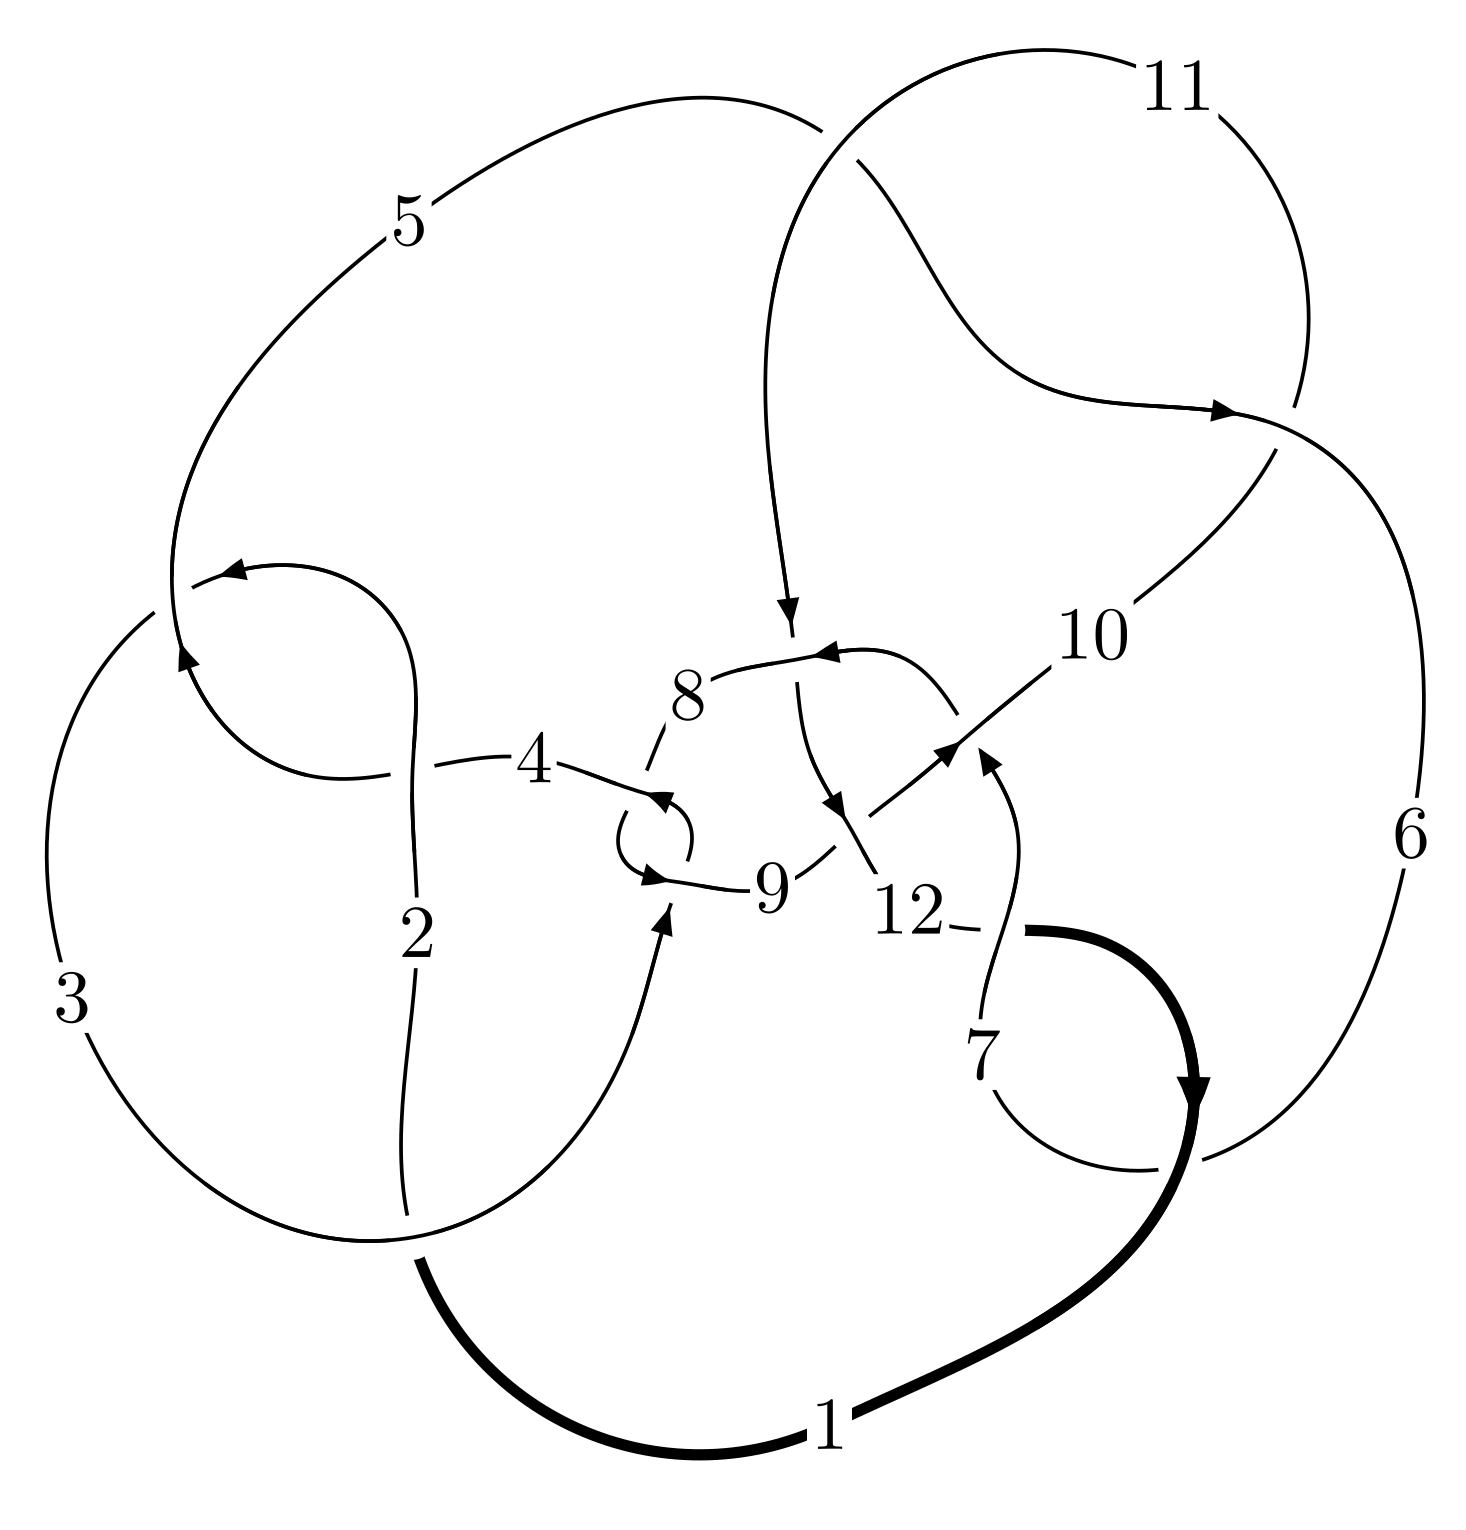
\includegraphics[width=112pt]{../../../GIT/diagram.site/Diagrams/png/963_12a_0162.png}\\
\ \ \ A knot diagram\footnotemark}&
\allowdisplaybreaks
\textbf{Linearized knot diagam} \\
\cline{2-2}
 &
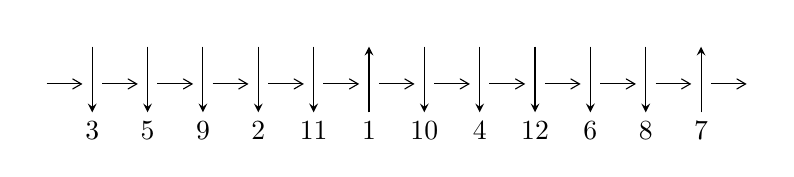
\begin{tikzpicture}[x=20pt, y=17pt]
	% nodes
	\node (C0) at (0, 0) {};
	\node (C1) at (1, 0) {};
	\node (C1U) at (1, +1) {};
	\node (C1D) at (1, -1) {3};

	\node (C2) at (2, 0) {};
	\node (C2U) at (2, +1) {};
	\node (C2D) at (2, -1) {5};

	\node (C3) at (3, 0) {};
	\node (C3U) at (3, +1) {};
	\node (C3D) at (3, -1) {9};

	\node (C4) at (4, 0) {};
	\node (C4U) at (4, +1) {};
	\node (C4D) at (4, -1) {2};

	\node (C5) at (5, 0) {};
	\node (C5U) at (5, +1) {};
	\node (C5D) at (5, -1) {11};

	\node (C6) at (6, 0) {};
	\node (C6U) at (6, +1) {};
	\node (C6D) at (6, -1) {1};

	\node (C7) at (7, 0) {};
	\node (C7U) at (7, +1) {};
	\node (C7D) at (7, -1) {10};

	\node (C8) at (8, 0) {};
	\node (C8U) at (8, +1) {};
	\node (C8D) at (8, -1) {4};

	\node (C9) at (9, 0) {};
	\node (C9U) at (9, +1) {};
	\node (C9D) at (9, -1) {12};

	\node (C10) at (10, 0) {};
	\node (C10U) at (10, +1) {};
	\node (C10D) at (10, -1) {6};

	\node (C11) at (11, 0) {};
	\node (C11U) at (11, +1) {};
	\node (C11D) at (11, -1) {8};

	\node (C12) at (12, 0) {};
	\node (C12U) at (12, +1) {};
	\node (C12D) at (12, -1) {7};
	\node (C13) at (13, 0) {};

	% arrows
	\draw[->,>={angle 60}]
	(C0) edge (C1) (C1) edge (C2) (C2) edge (C3) (C3) edge (C4) (C4) edge (C5) (C5) edge (C6) (C6) edge (C7) (C7) edge (C8) (C8) edge (C9) (C9) edge (C10) (C10) edge (C11) (C11) edge (C12) (C12) edge (C13) ;	\draw[->,>=stealth]
	(C1U) edge (C1D) (C2U) edge (C2D) (C3U) edge (C3D) (C4U) edge (C4D) (C5U) edge (C5D) (C6D) edge (C6U) (C7U) edge (C7D) (C8U) edge (C8D) (C9U) edge (C9D) (C10U) edge (C10D) (C11U) edge (C11D) (C12D) edge (C12U) ;
	\end{tikzpicture} \\
\hhline{~~} \\& 
\textbf{Solving Sequence} \\ \cline{2-2} 
 &
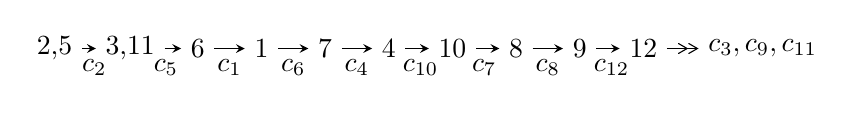
\begin{tikzpicture}[x=23pt, y=7pt]
	% node
	\node (A0) at (-1/8, 0) {2,5};
	\node (A1) at (17/16, 0) {3,11};
	\node (A2) at (17/8, 0) {6};
	\node (A3) at (25/8, 0) {1};
	\node (A4) at (33/8, 0) {7};
	\node (A5) at (41/8, 0) {4};
	\node (A6) at (49/8, 0) {10};
	\node (A7) at (57/8, 0) {8};
	\node (A8) at (65/8, 0) {9};
	\node (A9) at (73/8, 0) {12};
	\node (C1) at (1/2, -1) {$c_{2}$};
	\node (C2) at (13/8, -1) {$c_{5}$};
	\node (C3) at (21/8, -1) {$c_{1}$};
	\node (C4) at (29/8, -1) {$c_{6}$};
	\node (C5) at (37/8, -1) {$c_{4}$};
	\node (C6) at (45/8, -1) {$c_{10}$};
	\node (C7) at (53/8, -1) {$c_{7}$};
	\node (C8) at (61/8, -1) {$c_{8}$};
	\node (C9) at (69/8, -1) {$c_{12}$};
	\node (A10) at (11, 0) {$c_{3},c_{9},c_{11}$};

	% edge
	\draw[->,>=stealth]	
	(A0) edge (A1) (A1) edge (A2) (A2) edge (A3) (A3) edge (A4) (A4) edge (A5) (A5) edge (A6) (A6) edge (A7) (A7) edge (A8) (A8) edge (A9) ;
	\draw[->>,>={angle 60}]	
	(A9) edge (A10);
\end{tikzpicture} \\ 

\end{tabular} \\

\footnotetext{
The image of knot diagram is generated by the software ``\textbf{Draw programme}" developed by Andrew Bartholomew(\url{http://www.layer8.co.uk/maths/draw/index.htm\#Running-draw}), where we modified some parts for our purpose(\url{https://github.com/CATsTAILs/LinksPainter}).
}\phantom \\ \newline 
\centering \textbf{Ideals for irreducible components\footnotemark of $X_{\text{par}}$} 
 
\begin{align*}
I^u_{1}&=\langle 
1.29523\times10^{304} u^{152}-8.92919\times10^{305} u^{151}+\cdots+1.94694\times10^{303} b+3.53899\times10^{307},\\
\phantom{I^u_{1}}&\phantom{= \langle  }5.00929\times10^{304} u^{152}+5.88603\times10^{305} u^{151}+\cdots+2.72571\times10^{302} a+2.91301\times10^{305},\\
\phantom{I^u_{1}}&\phantom{= \langle  }u^{153}+14 u^{152}+\cdots-762 u-49\rangle \\
I^u_{2}&=\langle 
-7 u^{23}-26 u^{22}+\cdots+b-8,\;-6 u^{23}-18 u^{22}+\cdots+a-4,\;u^{24}+4 u^{23}+\cdots+3 u+1\rangle \\
I^u_{3}&=\langle 
a^8+2 a^6+a^5+4 a^4+3 a^3+5 a^2+7 b-9 a+6,\;a^9- a^8+2 a^7- a^6+3 a^5- a^4+2 a^3+a+1,\;u-1\rangle \\
\\
\end{align*}
\raggedright * 3 irreducible components of $\dim_{\mathbb{C}}=0$, with total 186 representations.\\
\footnotetext{All coefficients of polynomials are rational numbers. But the coefficients are sometimes approximated in decimal forms when there is not enough margin.}
\newpage
\renewcommand{\arraystretch}{1}
\centering \section*{I. $I^u_{1}= \langle 1.30\times10^{304} u^{152}-8.93\times10^{305} u^{151}+\cdots+1.95\times10^{303} b+3.54\times10^{307},\;5.01\times10^{304} u^{152}+5.89\times10^{305} u^{151}+\cdots+2.73\times10^{302} a+2.91\times10^{305},\;u^{153}+14 u^{152}+\cdots-762 u-49 \rangle$}
\flushleft \textbf{(i) Arc colorings}\\
\begin{tabular}{m{7pt} m{180pt} m{7pt} m{180pt} }
\flushright $a_{2}=$&$\begin{pmatrix}1\\0\end{pmatrix}$ \\
\flushright $a_{5}=$&$\begin{pmatrix}0\\u\end{pmatrix}$ \\
\flushright $a_{3}=$&$\begin{pmatrix}1\\u^2\end{pmatrix}$ \\
\flushright $a_{11}=$&$\begin{pmatrix}-183.779 u^{152}-2159.45 u^{151}+\cdots-7908.06 u-1068.72\\-6.65267 u^{152}+458.628 u^{151}+\cdots-255952. u-18177.2\end{pmatrix}$ \\
\flushright $a_{6}=$&$\begin{pmatrix}45.7365 u^{152}+309.760 u^{151}+\cdots+116257. u+8455.45\\616.534 u^{152}+7545.94 u^{151}+\cdots-118442. u-6864.99\end{pmatrix}$ \\
\flushright $a_{1}=$&$\begin{pmatrix}- u^2+1\\- u^4\end{pmatrix}$ \\
\flushright $a_{7}=$&$\begin{pmatrix}-446.080 u^{152}-6191.45 u^{151}+\cdots+446245. u+30706.7\\-74.8796 u^{152}-1734.74 u^{151}+\cdots+411019. u+29036.3\end{pmatrix}$ \\
\flushright $a_{4}=$&$\begin{pmatrix}u\\u\end{pmatrix}$ \\
\flushright $a_{10}=$&$\begin{pmatrix}504.654 u^{152}+6286.66 u^{151}+\cdots-160897. u-10329.5\\1128.83 u^{152}+14406.8 u^{151}+\cdots-512631. u-33700.1\end{pmatrix}$ \\
\flushright $a_{8}=$&$\begin{pmatrix}-220.118 u^{152}-2878.28 u^{151}+\cdots+137443. u+9289.07\\-350.744 u^{152}-4657.56 u^{151}+\cdots+250754. u+16977.6\end{pmatrix}$ \\
\flushright $a_{9}=$&$\begin{pmatrix}-296.996 u^{152}-3730.32 u^{151}+\cdots+106135. u+6864.24\\-427.622 u^{152}-5509.60 u^{151}+\cdots+219446. u+14552.8\end{pmatrix}$ \\
\flushright $a_{12}=$&$\begin{pmatrix}-632.625 u^{152}-8218.23 u^{151}+\cdots+354761. u+23565.6\\-617.458 u^{152}-8034.34 u^{151}+\cdots+357702. u+23903.3\end{pmatrix}$\\&\end{tabular}
\flushleft \textbf{(ii) Obstruction class $= -1$}\\~\\
\flushleft \textbf{(iii) Cusp Shapes $= -424.076 u^{152}-5406.81 u^{151}+\cdots+203917. u+13552.6$}\\~\\
\newpage\renewcommand{\arraystretch}{1}
\flushleft \textbf{(iv) u-Polynomials at the component}\newline \\
\begin{tabular}{m{50pt}|m{274pt}}
Crossings & \hspace{64pt}u-Polynomials at each crossing \\
\hline $$\begin{aligned}c_{1}\end{aligned}$$&$\begin{aligned}
&u^{153}+76 u^{152}+\cdots+169142 u+2401
\end{aligned}$\\
\hline $$\begin{aligned}c_{2},c_{4}\end{aligned}$$&$\begin{aligned}
&u^{153}-14 u^{152}+\cdots-762 u+49
\end{aligned}$\\
\hline $$\begin{aligned}c_{3},c_{8}\end{aligned}$$&$\begin{aligned}
&u^{153}- u^{152}+\cdots-100352 u+25088
\end{aligned}$\\
\hline $$\begin{aligned}c_{5},c_{10}\end{aligned}$$&$\begin{aligned}
&u^{153}+2 u^{152}+\cdots+1528 u+649
\end{aligned}$\\
\hline $$\begin{aligned}c_{6},c_{12}\end{aligned}$$&$\begin{aligned}
&u^{153}+3 u^{152}+\cdots+50071 u+3559
\end{aligned}$\\
\hline $$\begin{aligned}c_{7}\end{aligned}$$&$\begin{aligned}
&u^{153}-10 u^{152}+\cdots+14 u+17
\end{aligned}$\\
\hline $$\begin{aligned}c_{9}\end{aligned}$$&$\begin{aligned}
&u^{153}-20 u^{152}+\cdots+18213 u+14027
\end{aligned}$\\
\hline $$\begin{aligned}c_{11}\end{aligned}$$&$\begin{aligned}
&u^{153}- u^{152}+\cdots+118105 u+15199
\end{aligned}$\\
\hline
\end{tabular}\\~\\
\newpage\renewcommand{\arraystretch}{1}
\flushleft \textbf{(v) Riley Polynomials at the component}\newline \\
\begin{tabular}{m{50pt}|m{274pt}}
Crossings & \hspace{64pt}Riley Polynomials at each crossing \\
\hline $$\begin{aligned}c_{1}\end{aligned}$$&$\begin{aligned}
&y^{153}+16 y^{152}+\cdots+4705654178 y-5764801
\end{aligned}$\\
\hline $$\begin{aligned}c_{2},c_{4}\end{aligned}$$&$\begin{aligned}
&y^{153}-76 y^{152}+\cdots+169142 y-2401
\end{aligned}$\\
\hline $$\begin{aligned}c_{3},c_{8}\end{aligned}$$&$\begin{aligned}
&y^{153}+69 y^{152}+\cdots-16338911232 y-629407744
\end{aligned}$\\
\hline $$\begin{aligned}c_{5},c_{10}\end{aligned}$$&$\begin{aligned}
&y^{153}+96 y^{152}+\cdots-17206606 y-421201
\end{aligned}$\\
\hline $$\begin{aligned}c_{6},c_{12}\end{aligned}$$&$\begin{aligned}
&y^{153}+99 y^{152}+\cdots-548780483 y-12666481
\end{aligned}$\\
\hline $$\begin{aligned}c_{7}\end{aligned}$$&$\begin{aligned}
&y^{153}-8 y^{152}+\cdots-9698 y-289
\end{aligned}$\\
\hline $$\begin{aligned}c_{9}\end{aligned}$$&$\begin{aligned}
&y^{153}-40 y^{152}+\cdots+18060550885 y-196756729
\end{aligned}$\\
\hline $$\begin{aligned}c_{11}\end{aligned}$$&$\begin{aligned}
&y^{153}+3 y^{152}+\cdots-3235076783 y-231009601
\end{aligned}$\\
\hline
\end{tabular}\\~\\
\newpage\flushleft \textbf{(vi) Complex Volumes and Cusp Shapes}
$$\begin{array}{c|c|c}  
\text{Solutions to }I^u_{1}& \I (\text{vol} + \sqrt{-1}CS) & \text{Cusp shape}\\
 \hline 
\begin{aligned}
u &= -0.574594 + 0.816890 I \\
a &= \phantom{-}1.43644 - 0.31596 I \\
b &= \phantom{-}0.611437 - 0.397016 I\end{aligned}
 & \phantom{-}5.13882 + 1.56779 I & \phantom{-0.000000 } 0 \\ \hline\begin{aligned}
u &= -0.574594 - 0.816890 I \\
a &= \phantom{-}1.43644 + 0.31596 I \\
b &= \phantom{-}0.611437 + 0.397016 I\end{aligned}
 & \phantom{-}5.13882 - 1.56779 I & \phantom{-0.000000 } 0 \\ \hline\begin{aligned}
u &= \phantom{-}0.958484 + 0.278909 I \\
a &= \phantom{-}0.38766 + 1.64685 I \\
b &= \phantom{-}2.38666 + 0.30401 I\end{aligned}
 & \phantom{-}1.129760 - 0.814632 I & \phantom{-0.000000 } 0 \\ \hline\begin{aligned}
u &= \phantom{-}0.958484 - 0.278909 I \\
a &= \phantom{-}0.38766 - 1.64685 I \\
b &= \phantom{-}2.38666 - 0.30401 I\end{aligned}
 & \phantom{-}1.129760 + 0.814632 I & \phantom{-0.000000 } 0 \\ \hline\begin{aligned}
u &= -0.895884 + 0.430701 I \\
a &= -0.551403 - 0.393529 I \\
b &= -1.57433 + 0.45310 I\end{aligned}
 & -2.14959 + 1.73247 I & \phantom{-0.000000 } 0 \\ \hline\begin{aligned}
u &= -0.895884 - 0.430701 I \\
a &= -0.551403 + 0.393529 I \\
b &= -1.57433 - 0.45310 I\end{aligned}
 & -2.14959 - 1.73247 I & \phantom{-0.000000 } 0 \\ \hline\begin{aligned}
u &= -0.985972 + 0.213998 I \\
a &= \phantom{-}0.539482 + 1.196150 I \\
b &= \phantom{-}1.34686 + 1.00600 I\end{aligned}
 & -5.33229 - 6.54252 I & \phantom{-0.000000 } 0 \\ \hline\begin{aligned}
u &= -0.985972 - 0.213998 I \\
a &= \phantom{-}0.539482 - 1.196150 I \\
b &= \phantom{-}1.34686 - 1.00600 I\end{aligned}
 & -5.33229 + 6.54252 I & \phantom{-0.000000 } 0 \\ \hline\begin{aligned}
u &= -0.308239 + 0.976529 I \\
a &= \phantom{-}1.08835 - 1.00361 I \\
b &= \phantom{-}0.089777 + 0.592784 I\end{aligned}
 & \phantom{-}2.3368 - 14.2623 I & \phantom{-0.000000 } 0 \\ \hline\begin{aligned}
u &= -0.308239 - 0.976529 I \\
a &= \phantom{-}1.08835 + 1.00361 I \\
b &= \phantom{-}0.089777 - 0.592784 I\end{aligned}
 & \phantom{-}2.3368 + 14.2623 I & \phantom{-0.000000 } 0\\
 \hline 
 \end{array}$$\newpage$$\begin{array}{c|c|c}  
\text{Solutions to }I^u_{1}& \I (\text{vol} + \sqrt{-1}CS) & \text{Cusp shape}\\
 \hline 
\begin{aligned}
u &= -0.445994 + 0.851018 I \\
a &= -0.73156 + 1.41683 I \\
b &= \phantom{-}0.154985 - 0.466806 I\end{aligned}
 & \phantom{-}4.36623 - 5.28259 I & \phantom{-0.000000 } 0 \\ \hline\begin{aligned}
u &= -0.445994 - 0.851018 I \\
a &= -0.73156 - 1.41683 I \\
b &= \phantom{-}0.154985 + 0.466806 I\end{aligned}
 & \phantom{-}4.36623 + 5.28259 I & \phantom{-0.000000 } 0 \\ \hline\begin{aligned}
u &= \phantom{-}0.950665 + 0.433419 I \\
a &= \phantom{-}0.438661 - 0.209931 I \\
b &= \phantom{-}1.48917 - 0.57495 I\end{aligned}
 & -1.93090 - 3.15315 I & \phantom{-0.000000 } 0 \\ \hline\begin{aligned}
u &= \phantom{-}0.950665 - 0.433419 I \\
a &= \phantom{-}0.438661 + 0.209931 I \\
b &= \phantom{-}1.48917 + 0.57495 I\end{aligned}
 & -1.93090 + 3.15315 I & \phantom{-0.000000 } 0 \\ \hline\begin{aligned}
u &= \phantom{-}0.920630 + 0.495323 I \\
a &= \phantom{-}1.205590 + 0.584838 I \\
b &= \phantom{-}2.53864 - 0.21529 I\end{aligned}
 & -0.38761 - 5.07239 I & \phantom{-0.000000 } 0 \\ \hline\begin{aligned}
u &= \phantom{-}0.920630 - 0.495323 I \\
a &= \phantom{-}1.205590 - 0.584838 I \\
b &= \phantom{-}2.53864 + 0.21529 I\end{aligned}
 & -0.38761 + 5.07239 I & \phantom{-0.000000 } 0 \\ \hline\begin{aligned}
u &= -0.322725 + 0.895754 I \\
a &= -1.038100 + 0.891150 I \\
b &= \phantom{-}0.152242 - 0.790387 I\end{aligned}
 & \phantom{-}5.83587 - 7.72355 I & \phantom{-0.000000 } 0 \\ \hline\begin{aligned}
u &= -0.322725 - 0.895754 I \\
a &= -1.038100 - 0.891150 I \\
b &= \phantom{-}0.152242 + 0.790387 I\end{aligned}
 & \phantom{-}5.83587 + 7.72355 I & \phantom{-0.000000 } 0 \\ \hline\begin{aligned}
u &= \phantom{-}0.418416 + 0.967520 I \\
a &= -0.891483 - 0.133621 I \\
b &= -0.399415 + 0.176695 I\end{aligned}
 & -1.16480 - 4.56244 I & \phantom{-0.000000 } 0 \\ \hline\begin{aligned}
u &= \phantom{-}0.418416 - 0.967520 I \\
a &= -0.891483 + 0.133621 I \\
b &= -0.399415 - 0.176695 I\end{aligned}
 & -1.16480 + 4.56244 I & \phantom{-0.000000 } 0\\
 \hline 
 \end{array}$$\newpage$$\begin{array}{c|c|c}  
\text{Solutions to }I^u_{1}& \I (\text{vol} + \sqrt{-1}CS) & \text{Cusp shape}\\
 \hline 
\begin{aligned}
u &= -0.910466 + 0.237134 I \\
a &= \phantom{-}0.618889 + 1.147390 I \\
b &= \phantom{-}1.188320 + 0.395835 I\end{aligned}
 & -5.78318 + 2.01516 I & \phantom{-0.000000 } 0 \\ \hline\begin{aligned}
u &= -0.910466 - 0.237134 I \\
a &= \phantom{-}0.618889 - 1.147390 I \\
b &= \phantom{-}1.188320 - 0.395835 I\end{aligned}
 & -5.78318 - 2.01516 I & \phantom{-0.000000 } 0 \\ \hline\begin{aligned}
u &= \phantom{-}0.990973 + 0.383908 I \\
a &= -0.736554 - 1.003330 I \\
b &= -2.52442 - 1.13711 I\end{aligned}
 & \phantom{-}0.54761 - 1.44300 I & \phantom{-0.000000 } 0 \\ \hline\begin{aligned}
u &= \phantom{-}0.990973 - 0.383908 I \\
a &= -0.736554 + 1.003330 I \\
b &= -2.52442 + 1.13711 I\end{aligned}
 & \phantom{-}0.54761 + 1.44300 I & \phantom{-0.000000 } 0 \\ \hline\begin{aligned}
u &= -0.686108 + 0.634402 I \\
a &= -1.185060 - 0.533186 I \\
b &= -0.873123 + 0.960621 I\end{aligned}
 & \phantom{-}0.67913 + 5.24901 I & \phantom{-0.000000 } 0 \\ \hline\begin{aligned}
u &= -0.686108 - 0.634402 I \\
a &= -1.185060 + 0.533186 I \\
b &= -0.873123 - 0.960621 I\end{aligned}
 & \phantom{-}0.67913 - 5.24901 I & \phantom{-0.000000 } 0 \\ \hline\begin{aligned}
u &= \phantom{-}0.903188 + 0.238495 I \\
a &= -0.055343 - 0.756165 I \\
b &= -4.52323 + 0.01015 I\end{aligned}
 & -2.69283 + 2.12824 I & \phantom{-0.000000 } 0 \\ \hline\begin{aligned}
u &= \phantom{-}0.903188 - 0.238495 I \\
a &= -0.055343 + 0.756165 I \\
b &= -4.52323 - 0.01015 I\end{aligned}
 & -2.69283 - 2.12824 I & \phantom{-0.000000 } 0 \\ \hline\begin{aligned}
u &= -1.003950 + 0.371462 I \\
a &= -0.034393 - 0.897261 I \\
b &= -1.26131 - 1.05136 I\end{aligned}
 & \phantom{-}0.011275 - 0.515252 I & \phantom{-0.000000 } 0 \\ \hline\begin{aligned}
u &= -1.003950 - 0.371462 I \\
a &= -0.034393 + 0.897261 I \\
b &= -1.26131 + 1.05136 I\end{aligned}
 & \phantom{-}0.011275 + 0.515252 I & \phantom{-0.000000 } 0\\
 \hline 
 \end{array}$$\newpage$$\begin{array}{c|c|c}  
\text{Solutions to }I^u_{1}& \I (\text{vol} + \sqrt{-1}CS) & \text{Cusp shape}\\
 \hline 
\begin{aligned}
u &= -0.462720 + 0.973186 I \\
a &= -0.649975 + 0.436879 I \\
b &= -0.263586 - 0.603612 I\end{aligned}
 & \phantom{-}3.60458 - 2.74950 I & \phantom{-0.000000 } 0 \\ \hline\begin{aligned}
u &= -0.462720 - 0.973186 I \\
a &= -0.649975 - 0.436879 I \\
b &= -0.263586 + 0.603612 I\end{aligned}
 & \phantom{-}3.60458 + 2.74950 I & \phantom{-0.000000 } 0 \\ \hline\begin{aligned}
u &= \phantom{-}0.835570 + 0.687935 I \\
a &= \phantom{-}0.349315 + 0.614531 I \\
b &= \phantom{-}1.242750 + 0.025699 I\end{aligned}
 & -1.88517 - 2.34362 I & \phantom{-0.000000 } 0 \\ \hline\begin{aligned}
u &= \phantom{-}0.835570 - 0.687935 I \\
a &= \phantom{-}0.349315 - 0.614531 I \\
b &= \phantom{-}1.242750 - 0.025699 I\end{aligned}
 & -1.88517 + 2.34362 I & \phantom{-0.000000 } 0 \\ \hline\begin{aligned}
u &= \phantom{-}1.016760 + 0.370999 I \\
a &= \phantom{-}0.645130 + 0.786096 I \\
b &= \phantom{-}3.36215 - 1.03847 I\end{aligned}
 & -3.53913 - 4.44208 I & \phantom{-0.000000 } 0 \\ \hline\begin{aligned}
u &= \phantom{-}1.016760 - 0.370999 I \\
a &= \phantom{-}0.645130 - 0.786096 I \\
b &= \phantom{-}3.36215 + 1.03847 I\end{aligned}
 & -3.53913 + 4.44208 I & \phantom{-0.000000 } 0 \\ \hline\begin{aligned}
u &= -0.756138 + 0.780095 I \\
a &= \phantom{-}1.064490 - 0.701322 I \\
b &= \phantom{-}1.207020 - 0.635288 I\end{aligned}
 & \phantom{-}8.53653 + 4.24665 I & \phantom{-0.000000 } 0 \\ \hline\begin{aligned}
u &= -0.756138 - 0.780095 I \\
a &= \phantom{-}1.064490 + 0.701322 I \\
b &= \phantom{-}1.207020 + 0.635288 I\end{aligned}
 & \phantom{-}8.53653 - 4.24665 I & \phantom{-0.000000 } 0 \\ \hline\begin{aligned}
u &= -0.939531 + 0.552017 I \\
a &= -0.582454 - 1.069380 I \\
b &= -2.08714 - 0.73277 I\end{aligned}
 & -0.071240 - 0.591588 I & \phantom{-0.000000 } 0 \\ \hline\begin{aligned}
u &= -0.939531 - 0.552017 I \\
a &= -0.582454 + 1.069380 I \\
b &= -2.08714 + 0.73277 I\end{aligned}
 & -0.071240 + 0.591588 I & \phantom{-0.000000 } 0\\
 \hline 
 \end{array}$$\newpage$$\begin{array}{c|c|c}  
\text{Solutions to }I^u_{1}& \I (\text{vol} + \sqrt{-1}CS) & \text{Cusp shape}\\
 \hline 
\begin{aligned}
u &= \phantom{-}0.475132 + 0.764717 I \\
a &= \phantom{-}0.83450 + 1.24262 I \\
b &= \phantom{-}0.544227 - 0.336753 I\end{aligned}
 & -0.70902 + 7.98208 I & \phantom{-0.000000 } 0 \\ \hline\begin{aligned}
u &= \phantom{-}0.475132 - 0.764717 I \\
a &= \phantom{-}0.83450 - 1.24262 I \\
b &= \phantom{-}0.544227 + 0.336753 I\end{aligned}
 & -0.70902 - 7.98208 I & \phantom{-0.000000 } 0 \\ \hline\begin{aligned}
u &= -0.291130 + 1.063480 I \\
a &= \phantom{-}1.008020 - 0.522408 I \\
b &= \phantom{-}0.396508 + 0.228257 I\end{aligned}
 & \phantom{-}2.80976 - 4.80966 I & \phantom{-0.000000 } 0 \\ \hline\begin{aligned}
u &= -0.291130 - 1.063480 I \\
a &= \phantom{-}1.008020 + 0.522408 I \\
b &= \phantom{-}0.396508 - 0.228257 I\end{aligned}
 & \phantom{-}2.80976 + 4.80966 I & \phantom{-0.000000 } 0 \\ \hline\begin{aligned}
u &= -0.299280 + 0.841358 I \\
a &= -0.63160 - 1.34503 I \\
b &= -0.542959 + 0.482245 I\end{aligned}
 & -1.60886 - 7.51304 I & \phantom{-0.000000 } 0 \\ \hline\begin{aligned}
u &= -0.299280 - 0.841358 I \\
a &= -0.63160 + 1.34503 I \\
b &= -0.542959 - 0.482245 I\end{aligned}
 & -1.60886 + 7.51304 I & \phantom{-0.000000 } 0 \\ \hline\begin{aligned}
u &= -1.041590 + 0.376605 I \\
a &= \phantom{-}1.156170 - 0.184868 I \\
b &= \phantom{-}2.13045 - 0.50677 I\end{aligned}
 & -6.76823 + 0.15150 I & \phantom{-0.000000 } 0 \\ \hline\begin{aligned}
u &= -1.041590 - 0.376605 I \\
a &= \phantom{-}1.156170 + 0.184868 I \\
b &= \phantom{-}2.13045 + 0.50677 I\end{aligned}
 & -6.76823 - 0.15150 I & \phantom{-0.000000 } 0 \\ \hline\begin{aligned}
u &= \phantom{-}0.752593 + 0.475568 I \\
a &= -0.13687 - 1.44830 I \\
b &= -0.982498 - 0.298007 I\end{aligned}
 & \phantom{-}0.157068 + 1.043870 I & \phantom{-0.000000 } 0 \\ \hline\begin{aligned}
u &= \phantom{-}0.752593 - 0.475568 I \\
a &= -0.13687 + 1.44830 I \\
b &= -0.982498 + 0.298007 I\end{aligned}
 & \phantom{-}0.157068 - 1.043870 I & \phantom{-0.000000 } 0\\
 \hline 
 \end{array}$$\newpage$$\begin{array}{c|c|c}  
\text{Solutions to }I^u_{1}& \I (\text{vol} + \sqrt{-1}CS) & \text{Cusp shape}\\
 \hline 
\begin{aligned}
u &= \phantom{-}1.086180 + 0.249085 I \\
a &= -0.209147 + 0.943972 I \\
b &= -1.187340 - 0.203491 I\end{aligned}
 & -3.84037 + 2.35778 I & \phantom{-0.000000 } 0 \\ \hline\begin{aligned}
u &= \phantom{-}1.086180 - 0.249085 I \\
a &= -0.209147 - 0.943972 I \\
b &= -1.187340 + 0.203491 I\end{aligned}
 & -3.84037 - 2.35778 I & \phantom{-0.000000 } 0 \\ \hline\begin{aligned}
u &= -0.547399 + 0.690954 I \\
a &= \phantom{-}0.807072 + 0.396069 I \\
b &= \phantom{-}0.708380 - 0.436182 I\end{aligned}
 & \phantom{-}3.19945 + 0.72226 I & \phantom{-0.000000 } 0 \\ \hline\begin{aligned}
u &= -0.547399 - 0.690954 I \\
a &= \phantom{-}0.807072 - 0.396069 I \\
b &= \phantom{-}0.708380 + 0.436182 I\end{aligned}
 & \phantom{-}3.19945 - 0.72226 I & \phantom{-0.000000 } 0 \\ \hline\begin{aligned}
u &= -0.421737 + 0.773562 I \\
a &= \phantom{-}0.441743 + 0.638691 I \\
b &= \phantom{-}0.338898 - 0.840790 I\end{aligned}
 & \phantom{-}2.45307 - 3.31889 I & \phantom{-0.000000 } 0 \\ \hline\begin{aligned}
u &= -0.421737 - 0.773562 I \\
a &= \phantom{-}0.441743 - 0.638691 I \\
b &= \phantom{-}0.338898 + 0.840790 I\end{aligned}
 & \phantom{-}2.45307 + 3.31889 I & \phantom{-0.000000 } 0 \\ \hline\begin{aligned}
u &= -0.799180 + 0.340969 I \\
a &= -0.448563 + 0.709569 I \\
b &= -0.320889 + 1.267110 I\end{aligned}
 & \phantom{-}0.76492 + 3.31721 I & \phantom{-0.000000 } 0 \\ \hline\begin{aligned}
u &= -0.799180 - 0.340969 I \\
a &= -0.448563 - 0.709569 I \\
b &= -0.320889 - 1.267110 I\end{aligned}
 & \phantom{-}0.76492 - 3.31721 I & \phantom{-0.000000 } 0 \\ \hline\begin{aligned}
u &= \phantom{-}0.857796 + 0.098270 I \\
a &= -0.665279 - 0.516870 I \\
b &= \phantom{-}0.12954 - 2.58752 I\end{aligned}
 & -2.79806 - 3.16139 I & \phantom{-0.000000 } 0 \\ \hline\begin{aligned}
u &= \phantom{-}0.857796 - 0.098270 I \\
a &= -0.665279 + 0.516870 I \\
b &= \phantom{-}0.12954 + 2.58752 I\end{aligned}
 & -2.79806 + 3.16139 I & \phantom{-0.000000 } 0\\
 \hline 
 \end{array}$$\newpage$$\begin{array}{c|c|c}  
\text{Solutions to }I^u_{1}& \I (\text{vol} + \sqrt{-1}CS) & \text{Cusp shape}\\
 \hline 
\begin{aligned}
u &= -0.880694 + 0.741742 I \\
a &= -0.677390 + 1.004890 I \\
b &= -0.475986 + 0.314668 I\end{aligned}
 & \phantom{-}8.17021 + 1.41350 I & \phantom{-0.000000 } 0 \\ \hline\begin{aligned}
u &= -0.880694 - 0.741742 I \\
a &= -0.677390 - 1.004890 I \\
b &= -0.475986 - 0.314668 I\end{aligned}
 & \phantom{-}8.17021 - 1.41350 I & \phantom{-0.000000 } 0 \\ \hline\begin{aligned}
u &= \phantom{-}1.141200 + 0.200987 I \\
a &= -0.020466 - 1.001250 I \\
b &= -0.29566 - 2.51930 I\end{aligned}
 & \phantom{-}0.059344 - 0.653379 I & \phantom{-0.000000 } 0 \\ \hline\begin{aligned}
u &= \phantom{-}1.141200 - 0.200987 I \\
a &= -0.020466 + 1.001250 I \\
b &= -0.29566 + 2.51930 I\end{aligned}
 & \phantom{-}0.059344 + 0.653379 I & \phantom{-0.000000 } 0 \\ \hline\begin{aligned}
u &= -0.415285 + 0.729352 I \\
a &= \phantom{-}1.21677 - 1.36665 I \\
b &= -0.363475 + 0.196159 I\end{aligned}
 & \phantom{-}4.66993 - 1.60864 I & \phantom{-0.000000 } 0 \\ \hline\begin{aligned}
u &= -0.415285 - 0.729352 I \\
a &= \phantom{-}1.21677 + 1.36665 I \\
b &= -0.363475 - 0.196159 I\end{aligned}
 & \phantom{-}4.66993 + 1.60864 I & \phantom{-0.000000 } 0 \\ \hline\begin{aligned}
u &= -0.513574 + 0.661509 I \\
a &= \phantom{-}0.854458 - 0.718443 I \\
b &= \phantom{-}0.264014 + 1.180200 I\end{aligned}
 & \phantom{-}1.15055 + 2.63661 I & \phantom{-0.000000 } 0 \\ \hline\begin{aligned}
u &= -0.513574 - 0.661509 I \\
a &= \phantom{-}0.854458 + 0.718443 I \\
b &= \phantom{-}0.264014 - 1.180200 I\end{aligned}
 & \phantom{-}1.15055 - 2.63661 I & \phantom{-0.000000 } 0 \\ \hline\begin{aligned}
u &= -1.128740 + 0.303775 I \\
a &= \phantom{-}0.718205 - 0.479306 I \\
b &= \phantom{-}1.17724 - 0.86002 I\end{aligned}
 & -6.10563 + 7.70875 I & \phantom{-0.000000 } 0 \\ \hline\begin{aligned}
u &= -1.128740 - 0.303775 I \\
a &= \phantom{-}0.718205 + 0.479306 I \\
b &= \phantom{-}1.17724 + 0.86002 I\end{aligned}
 & -6.10563 - 7.70875 I & \phantom{-0.000000 } 0\\
 \hline 
 \end{array}$$\newpage$$\begin{array}{c|c|c}  
\text{Solutions to }I^u_{1}& \I (\text{vol} + \sqrt{-1}CS) & \text{Cusp shape}\\
 \hline 
\begin{aligned}
u &= -0.473091 + 0.682038 I \\
a &= -1.92664 + 0.94089 I \\
b &= -0.707865 + 0.663983 I\end{aligned}
 & \phantom{-}5.01099 - 0.58946 I & \phantom{-0.000000 } 0 \\ \hline\begin{aligned}
u &= -0.473091 - 0.682038 I \\
a &= -1.92664 - 0.94089 I \\
b &= -0.707865 - 0.663983 I\end{aligned}
 & \phantom{-}5.01099 + 0.58946 I & \phantom{-0.000000 } 0 \\ \hline\begin{aligned}
u &= -1.053300 + 0.514235 I \\
a &= -0.094594 - 1.058760 I \\
b &= -1.47704 - 0.34370 I\end{aligned}
 & -2.51484 + 2.05166 I & \phantom{-0.000000 } 0 \\ \hline\begin{aligned}
u &= -1.053300 - 0.514235 I \\
a &= -0.094594 + 1.058760 I \\
b &= -1.47704 + 0.34370 I\end{aligned}
 & -2.51484 - 2.05166 I & \phantom{-0.000000 } 0 \\ \hline\begin{aligned}
u &= -1.022370 + 0.574994 I \\
a &= \phantom{-}0.306223 + 0.756673 I \\
b &= \phantom{-}1.176480 + 0.613540 I\end{aligned}
 & \phantom{-}1.78661 + 4.16402 I & \phantom{-0.000000 } 0 \\ \hline\begin{aligned}
u &= -1.022370 - 0.574994 I \\
a &= \phantom{-}0.306223 - 0.756673 I \\
b &= \phantom{-}1.176480 - 0.613540 I\end{aligned}
 & \phantom{-}1.78661 - 4.16402 I & \phantom{-0.000000 } 0 \\ \hline\begin{aligned}
u &= \phantom{-}1.052340 + 0.530022 I \\
a &= \phantom{-}0.759606 + 0.722009 I \\
b &= \phantom{-}2.62643 + 1.01096 I\end{aligned}
 & \phantom{-}1.21069 - 6.89643 I & \phantom{-0.000000 } 0 \\ \hline\begin{aligned}
u &= \phantom{-}1.052340 - 0.530022 I \\
a &= \phantom{-}0.759606 - 0.722009 I \\
b &= \phantom{-}2.62643 - 1.01096 I\end{aligned}
 & \phantom{-}1.21069 + 6.89643 I & \phantom{-0.000000 } 0 \\ \hline\begin{aligned}
u &= \phantom{-}1.074240 + 0.485277 I \\
a &= -0.864128 + 0.597591 I \\
b &= -1.51424 + 0.86371 I\end{aligned}
 & -5.98888 - 6.70269 I & \phantom{-0.000000 } 0 \\ \hline\begin{aligned}
u &= \phantom{-}1.074240 - 0.485277 I \\
a &= -0.864128 - 0.597591 I \\
b &= -1.51424 - 0.86371 I\end{aligned}
 & -5.98888 + 6.70269 I & \phantom{-0.000000 } 0\\
 \hline 
 \end{array}$$\newpage$$\begin{array}{c|c|c}  
\text{Solutions to }I^u_{1}& \I (\text{vol} + \sqrt{-1}CS) & \text{Cusp shape}\\
 \hline 
\begin{aligned}
u &= -0.380909 + 0.726311 I \\
a &= -1.073540 + 0.909998 I \\
b &= -1.047390 - 0.527334 I\end{aligned}
 & \phantom{-}0.49834 - 4.72614 I & \phantom{-0.000000 } 0 \\ \hline\begin{aligned}
u &= -0.380909 - 0.726311 I \\
a &= -1.073540 - 0.909998 I \\
b &= -1.047390 + 0.527334 I\end{aligned}
 & \phantom{-}0.49834 + 4.72614 I & \phantom{-0.000000 } 0 \\ \hline\begin{aligned}
u &= -1.034590 + 0.568304 I \\
a &= -0.512156 + 0.536550 I \\
b &= -2.40744 + 0.91946 I\end{aligned}
 & -0.38974 + 2.15739 I & \phantom{-0.000000 } 0 \\ \hline\begin{aligned}
u &= -1.034590 - 0.568304 I \\
a &= -0.512156 - 0.536550 I \\
b &= -2.40744 - 0.91946 I\end{aligned}
 & -0.38974 - 2.15739 I & \phantom{-0.000000 } 0 \\ \hline\begin{aligned}
u &= \phantom{-}1.175560 + 0.134803 I \\
a &= -0.399314 + 0.105905 I \\
b &= -1.99799 - 0.23490 I\end{aligned}
 & -2.73096 + 1.04396 I & \phantom{-0.000000 } 0 \\ \hline\begin{aligned}
u &= \phantom{-}1.175560 - 0.134803 I \\
a &= -0.399314 - 0.105905 I \\
b &= -1.99799 + 0.23490 I\end{aligned}
 & -2.73096 - 1.04396 I & \phantom{-0.000000 } 0 \\ \hline\begin{aligned}
u &= -1.060810 + 0.573324 I \\
a &= \phantom{-}0.59956 - 1.45513 I \\
b &= \phantom{-}0.58157 - 1.65500 I\end{aligned}
 & \phantom{-}3.27382 + 5.45616 I & \phantom{-0.000000 } 0 \\ \hline\begin{aligned}
u &= -1.060810 - 0.573324 I \\
a &= \phantom{-}0.59956 + 1.45513 I \\
b &= \phantom{-}0.58157 + 1.65500 I\end{aligned}
 & \phantom{-}3.27382 - 5.45616 I & \phantom{-0.000000 } 0 \\ \hline\begin{aligned}
u &= \phantom{-}1.224400 + 0.068741 I \\
a &= -0.532926 + 0.902798 I \\
b &= -1.92312 + 1.84736 I\end{aligned}
 & -1.47879 + 2.88577 I & \phantom{-0.000000 } 0 \\ \hline\begin{aligned}
u &= \phantom{-}1.224400 - 0.068741 I \\
a &= -0.532926 - 0.902798 I \\
b &= -1.92312 - 1.84736 I\end{aligned}
 & -1.47879 - 2.88577 I & \phantom{-0.000000 } 0\\
 \hline 
 \end{array}$$\newpage$$\begin{array}{c|c|c}  
\text{Solutions to }I^u_{1}& \I (\text{vol} + \sqrt{-1}CS) & \text{Cusp shape}\\
 \hline 
\begin{aligned}
u &= -0.863443 + 0.872751 I \\
a &= -0.959659 + 0.533981 I \\
b &= -0.949387 + 0.408983 I\end{aligned}
 & \phantom{-}6.11189 + 9.64087 I & \phantom{-0.000000 } 0 \\ \hline\begin{aligned}
u &= -0.863443 - 0.872751 I \\
a &= -0.959659 - 0.533981 I \\
b &= -0.949387 - 0.408983 I\end{aligned}
 & \phantom{-}6.11189 - 9.64087 I & \phantom{-0.000000 } 0 \\ \hline\begin{aligned}
u &= \phantom{-}0.739678 + 0.219151 I \\
a &= \phantom{-}0.400872 - 0.401997 I \\
b &= -0.135479 - 0.086416 I\end{aligned}
 & -0.941917 - 0.128738 I & \phantom{-0.000000 } 0 \\ \hline\begin{aligned}
u &= \phantom{-}0.739678 - 0.219151 I \\
a &= \phantom{-}0.400872 + 0.401997 I \\
b &= -0.135479 + 0.086416 I\end{aligned}
 & -0.941917 + 0.128738 I & \phantom{-0.000000 } 0 \\ \hline\begin{aligned}
u &= -1.035830 + 0.669437 I \\
a &= -0.331350 + 1.132300 I \\
b &= -0.187671 + 1.352810 I\end{aligned}
 & \phantom{-}3.75333 + 3.98207 I & \phantom{-0.000000 } 0 \\ \hline\begin{aligned}
u &= -1.035830 - 0.669437 I \\
a &= -0.331350 - 1.132300 I \\
b &= -0.187671 - 1.352810 I\end{aligned}
 & \phantom{-}3.75333 - 3.98207 I & \phantom{-0.000000 } 0 \\ \hline\begin{aligned}
u &= -1.089530 + 0.585328 I \\
a &= -0.974000 + 0.715575 I \\
b &= -2.17476 + 1.70665 I\end{aligned}
 & \phantom{-}2.69237 + 6.63075 I & \phantom{-0.000000 } 0 \\ \hline\begin{aligned}
u &= -1.089530 - 0.585328 I \\
a &= -0.974000 - 0.715575 I \\
b &= -2.17476 - 1.70665 I\end{aligned}
 & \phantom{-}2.69237 - 6.63075 I & \phantom{-0.000000 } 0 \\ \hline\begin{aligned}
u &= -0.837975 + 0.909716 I \\
a &= \phantom{-}0.587194 - 0.809108 I \\
b &= \phantom{-}0.504659 - 0.451647 I\end{aligned}
 & \phantom{-}6.21066 - 3.22971 I & \phantom{-0.000000 } 0 \\ \hline\begin{aligned}
u &= -0.837975 - 0.909716 I \\
a &= \phantom{-}0.587194 + 0.809108 I \\
b &= \phantom{-}0.504659 + 0.451647 I\end{aligned}
 & \phantom{-}6.21066 + 3.22971 I & \phantom{-0.000000 } 0\\
 \hline 
 \end{array}$$\newpage$$\begin{array}{c|c|c}  
\text{Solutions to }I^u_{1}& \I (\text{vol} + \sqrt{-1}CS) & \text{Cusp shape}\\
 \hline 
\begin{aligned}
u &= -0.099158 + 0.756498 I \\
a &= \phantom{-}0.592396 + 0.050813 I \\
b &= -0.458333 - 0.104453 I\end{aligned}
 & -1.64798 - 2.66834 I & \phantom{-0.000000 } 0 \\ \hline\begin{aligned}
u &= -0.099158 - 0.756498 I \\
a &= \phantom{-}0.592396 - 0.050813 I \\
b &= -0.458333 + 0.104453 I\end{aligned}
 & -1.64798 + 2.66834 I & \phantom{-0.000000 } 0 \\ \hline\begin{aligned}
u &= \phantom{-}1.083140 + 0.603801 I \\
a &= -0.966437 - 0.669674 I \\
b &= -2.47668 - 0.63380 I\end{aligned}
 & -2.53615 - 13.16840 I & \phantom{-0.000000 } 0 \\ \hline\begin{aligned}
u &= \phantom{-}1.083140 - 0.603801 I \\
a &= -0.966437 + 0.669674 I \\
b &= -2.47668 + 0.63380 I\end{aligned}
 & -2.53615 + 13.16840 I & \phantom{-0.000000 } 0 \\ \hline\begin{aligned}
u &= -1.104090 + 0.571992 I \\
a &= \phantom{-}0.689921 - 0.744783 I \\
b &= \phantom{-}2.26823 - 0.25739 I\end{aligned}
 & -1.62186 + 9.68707 I & \phantom{-0.000000 } 0 \\ \hline\begin{aligned}
u &= -1.104090 - 0.571992 I \\
a &= \phantom{-}0.689921 + 0.744783 I \\
b &= \phantom{-}2.26823 + 0.25739 I\end{aligned}
 & -1.62186 - 9.68707 I & \phantom{-0.000000 } 0 \\ \hline\begin{aligned}
u &= -1.093210 + 0.599223 I \\
a &= \phantom{-}0.377768 + 0.440427 I \\
b &= \phantom{-}1.91811 + 0.21693 I\end{aligned}
 & \phantom{-}0.47061 + 8.49310 I & \phantom{-0.000000 } 0 \\ \hline\begin{aligned}
u &= -1.093210 - 0.599223 I \\
a &= \phantom{-}0.377768 - 0.440427 I \\
b &= \phantom{-}1.91811 - 0.21693 I\end{aligned}
 & \phantom{-}0.47061 - 8.49310 I & \phantom{-0.000000 } 0 \\ \hline\begin{aligned}
u &= \phantom{-}1.181270 + 0.402814 I \\
a &= -0.338281 - 0.206291 I \\
b &= -0.731939 - 1.066440 I\end{aligned}
 & -5.37187 - 1.31466 I & \phantom{-0.000000 } 0 \\ \hline\begin{aligned}
u &= \phantom{-}1.181270 - 0.402814 I \\
a &= -0.338281 + 0.206291 I \\
b &= -0.731939 + 1.066440 I\end{aligned}
 & -5.37187 + 1.31466 I & \phantom{-0.000000 } 0\\
 \hline 
 \end{array}$$\newpage$$\begin{array}{c|c|c}  
\text{Solutions to }I^u_{1}& \I (\text{vol} + \sqrt{-1}CS) & \text{Cusp shape}\\
 \hline 
\begin{aligned}
u &= \phantom{-}1.193610 + 0.397425 I \\
a &= \phantom{-}0.049032 - 0.338911 I \\
b &= \phantom{-}0.31645 - 1.38718 I\end{aligned}
 & -5.39360 - 1.42120 I & \phantom{-0.000000 } 0 \\ \hline\begin{aligned}
u &= \phantom{-}1.193610 - 0.397425 I \\
a &= \phantom{-}0.049032 + 0.338911 I \\
b &= \phantom{-}0.31645 + 1.38718 I\end{aligned}
 & -5.39360 + 1.42120 I & \phantom{-0.000000 } 0 \\ \hline\begin{aligned}
u &= -0.143355 + 0.717544 I \\
a &= \phantom{-}0.544841 - 0.795646 I \\
b &= -0.615379 + 0.090988 I\end{aligned}
 & -1.61580 - 2.44952 I & \phantom{-0.000000 } 0 \\ \hline\begin{aligned}
u &= -0.143355 - 0.717544 I \\
a &= \phantom{-}0.544841 + 0.795646 I \\
b &= -0.615379 - 0.090988 I\end{aligned}
 & -1.61580 + 2.44952 I & \phantom{-0.000000 } 0 \\ \hline\begin{aligned}
u &= \phantom{-}1.243180 + 0.255001 I \\
a &= \phantom{-}0.908613 + 0.036004 I \\
b &= \phantom{-}2.70401 - 0.44908 I\end{aligned}
 & -6.54190 + 4.09896 I & \phantom{-0.000000 } 0 \\ \hline\begin{aligned}
u &= \phantom{-}1.243180 - 0.255001 I \\
a &= \phantom{-}0.908613 - 0.036004 I \\
b &= \phantom{-}2.70401 + 0.44908 I\end{aligned}
 & -6.54190 - 4.09896 I & \phantom{-0.000000 } 0 \\ \hline\begin{aligned}
u &= -1.163740 + 0.522058 I \\
a &= -0.577269 - 0.000165 I \\
b &= -1.34147 + 0.78759 I\end{aligned}
 & -4.47893 + 7.12118 I & \phantom{-0.000000 } 0 \\ \hline\begin{aligned}
u &= -1.163740 - 0.522058 I \\
a &= -0.577269 + 0.000165 I \\
b &= -1.34147 - 0.78759 I\end{aligned}
 & -4.47893 - 7.12118 I & \phantom{-0.000000 } 0 \\ \hline\begin{aligned}
u &= -1.182340 + 0.490261 I \\
a &= -0.088343 + 0.277555 I \\
b &= \phantom{-}0.056302 + 1.177490 I\end{aligned}
 & -4.78165 + 7.26278 I & \phantom{-0.000000 } 0 \\ \hline\begin{aligned}
u &= -1.182340 - 0.490261 I \\
a &= -0.088343 - 0.277555 I \\
b &= \phantom{-}0.056302 - 1.177490 I\end{aligned}
 & -4.78165 - 7.26278 I & \phantom{-0.000000 } 0\\
 \hline 
 \end{array}$$\newpage$$\begin{array}{c|c|c}  
\text{Solutions to }I^u_{1}& \I (\text{vol} + \sqrt{-1}CS) & \text{Cusp shape}\\
 \hline 
\begin{aligned}
u &= -1.114330 + 0.637212 I \\
a &= \phantom{-}1.141340 - 0.448009 I \\
b &= \phantom{-}2.81103 - 1.10389 I\end{aligned}
 & \phantom{-}2.35547 + 10.80480 I & \phantom{-0.000000 } 0 \\ \hline\begin{aligned}
u &= -1.114330 - 0.637212 I \\
a &= \phantom{-}1.141340 + 0.448009 I \\
b &= \phantom{-}2.81103 + 1.10389 I\end{aligned}
 & \phantom{-}2.35547 - 10.80480 I & \phantom{-0.000000 } 0 \\ \hline\begin{aligned}
u &= \phantom{-}0.453306 + 0.551100 I \\
a &= -1.02786 - 1.33674 I \\
b &= -0.366857 + 0.794960 I\end{aligned}
 & \phantom{-}2.95829 + 2.47842 I & \phantom{-0.000000 } 0 \\ \hline\begin{aligned}
u &= \phantom{-}0.453306 - 0.551100 I \\
a &= -1.02786 + 1.33674 I \\
b &= -0.366857 - 0.794960 I\end{aligned}
 & \phantom{-}2.95829 - 2.47842 I & \phantom{-0.000000 } 0 \\ \hline\begin{aligned}
u &= \phantom{-}1.061580 + 0.729490 I \\
a &= -0.647723 - 0.556979 I \\
b &= -1.367820 - 0.089761 I\end{aligned}
 & -2.44919 - 3.44783 I & \phantom{-0.000000 } 0 \\ \hline\begin{aligned}
u &= \phantom{-}1.061580 - 0.729490 I \\
a &= -0.647723 + 0.556979 I \\
b &= -1.367820 + 0.089761 I\end{aligned}
 & -2.44919 + 3.44783 I & \phantom{-0.000000 } 0 \\ \hline\begin{aligned}
u &= \phantom{-}1.278810 + 0.211421 I \\
a &= -0.133232 + 0.909955 I \\
b &= -1.43070 + 1.65004 I\end{aligned}
 & \phantom{-}0.46000 + 4.24652 I & \phantom{-0.000000 } 0 \\ \hline\begin{aligned}
u &= \phantom{-}1.278810 - 0.211421 I \\
a &= -0.133232 - 0.909955 I \\
b &= -1.43070 - 1.65004 I\end{aligned}
 & \phantom{-}0.46000 - 4.24652 I & \phantom{-0.000000 } 0 \\ \hline\begin{aligned}
u &= -1.162650 + 0.587085 I \\
a &= -0.895914 - 0.642965 I \\
b &= -2.32771 - 0.50967 I\end{aligned}
 & -4.17318 + 12.79720 I & \phantom{-0.000000 } 0 \\ \hline\begin{aligned}
u &= -1.162650 - 0.587085 I \\
a &= -0.895914 + 0.642965 I \\
b &= -2.32771 + 0.50967 I\end{aligned}
 & -4.17318 - 12.79720 I & \phantom{-0.000000 } 0\\
 \hline 
 \end{array}$$\newpage$$\begin{array}{c|c|c}  
\text{Solutions to }I^u_{1}& \I (\text{vol} + \sqrt{-1}CS) & \text{Cusp shape}\\
 \hline 
\begin{aligned}
u &= -1.175180 + 0.608421 I \\
a &= \phantom{-}0.765208 - 0.611140 I \\
b &= \phantom{-}2.49847 - 1.55285 I\end{aligned}
 & \phantom{-}3.26481 + 13.23710 I & \phantom{-0.000000 } 0 \\ \hline\begin{aligned}
u &= -1.175180 - 0.608421 I \\
a &= \phantom{-}0.765208 + 0.611140 I \\
b &= \phantom{-}2.49847 + 1.55285 I\end{aligned}
 & \phantom{-}3.26481 - 13.23710 I & \phantom{-0.000000 } 0 \\ \hline\begin{aligned}
u &= -1.145890 + 0.676573 I \\
a &= \phantom{-}0.473936 - 0.365803 I \\
b &= \phantom{-}1.81755 - 0.55926 I\end{aligned}
 & \phantom{-}1.49037 + 8.72661 I & \phantom{-0.000000 } 0 \\ \hline\begin{aligned}
u &= -1.145890 - 0.676573 I \\
a &= \phantom{-}0.473936 + 0.365803 I \\
b &= \phantom{-}1.81755 + 0.55926 I\end{aligned}
 & \phantom{-}1.49037 - 8.72661 I & \phantom{-0.000000 } 0 \\ \hline\begin{aligned}
u &= -0.425630 + 0.481298 I \\
a &= -1.71107 + 0.19286 I \\
b &= -1.03407 + 1.24694 I\end{aligned}
 & -0.70464 + 2.18373 I & \phantom{-0.000000 } 0 \\ \hline\begin{aligned}
u &= -0.425630 - 0.481298 I \\
a &= -1.71107 - 0.19286 I \\
b &= -1.03407 - 1.24694 I\end{aligned}
 & -0.70464 - 2.18373 I & \phantom{-0.000000 } 0 \\ \hline\begin{aligned}
u &= -1.210940 + 0.629035 I \\
a &= -0.928344 + 0.663982 I \\
b &= -2.61075 + 1.33342 I\end{aligned}
 & -0.4238 + 20.0703 I & \phantom{-0.000000 } 0 \\ \hline\begin{aligned}
u &= -1.210940 - 0.629035 I \\
a &= -0.928344 - 0.663982 I \\
b &= -2.61075 - 1.33342 I\end{aligned}
 & -0.4238 - 20.0703 I & \phantom{-0.000000 } 0 \\ \hline\begin{aligned}
u &= \phantom{-}1.366400 + 0.224104 I \\
a &= \phantom{-}0.295360 - 0.972105 I \\
b &= \phantom{-}1.31293 - 1.54767 I\end{aligned}
 & -3.40243 + 10.22740 I & \phantom{-0.000000 } 0 \\ \hline\begin{aligned}
u &= \phantom{-}1.366400 - 0.224104 I \\
a &= \phantom{-}0.295360 + 0.972105 I \\
b &= \phantom{-}1.31293 + 1.54767 I\end{aligned}
 & -3.40243 - 10.22740 I & \phantom{-0.000000 } 0\\
 \hline 
 \end{array}$$\newpage$$\begin{array}{c|c|c}  
\text{Solutions to }I^u_{1}& \I (\text{vol} + \sqrt{-1}CS) & \text{Cusp shape}\\
 \hline 
\begin{aligned}
u &= -1.232330 + 0.644358 I \\
a &= -0.668575 + 0.689519 I \\
b &= -1.77944 + 0.95139 I\end{aligned}
 & -0.09625 + 10.86920 I & \phantom{-0.000000 } 0 \\ \hline\begin{aligned}
u &= -1.232330 - 0.644358 I \\
a &= -0.668575 - 0.689519 I \\
b &= -1.77944 - 0.95139 I\end{aligned}
 & -0.09625 - 10.86920 I & \phantom{-0.000000 } 0 \\ \hline\begin{aligned}
u &= \phantom{-}0.229915 + 0.531966 I \\
a &= -1.06334 + 1.25276 I \\
b &= -0.150349 + 0.347476 I\end{aligned}
 & -3.73555 + 2.61983 I & -8.00000 + 0. I\phantom{ +0.000000I} \\ \hline\begin{aligned}
u &= \phantom{-}0.229915 - 0.531966 I \\
a &= -1.06334 - 1.25276 I \\
b &= -0.150349 - 0.347476 I\end{aligned}
 & -3.73555 - 2.61983 I & -8.00000 + 0. I\phantom{ +0.000000I} \\ \hline\begin{aligned}
u &= \phantom{-}1.43890 + 0.08829 I \\
a &= \phantom{-}0.154398 - 0.639808 I \\
b &= \phantom{-}0.223053 - 0.509205 I\end{aligned}
 & -3.80031 + 0.34121 I & \phantom{-0.000000 } 0 \\ \hline\begin{aligned}
u &= \phantom{-}1.43890 - 0.08829 I \\
a &= \phantom{-}0.154398 + 0.639808 I \\
b &= \phantom{-}0.223053 + 0.509205 I\end{aligned}
 & -3.80031 - 0.34121 I & \phantom{-0.000000 } 0 \\ \hline\begin{aligned}
u &= \phantom{-}0.260834 + 0.419052 I \\
a &= \phantom{-}2.03463 + 1.18472 I \\
b &= \phantom{-}0.391031 - 0.543122 I\end{aligned}
 & \phantom{-}2.58263 - 1.72264 I & -1.48426 + 4.56743 I \\ \hline\begin{aligned}
u &= \phantom{-}0.260834 - 0.419052 I \\
a &= \phantom{-}2.03463 - 1.18472 I \\
b &= \phantom{-}0.391031 + 0.543122 I\end{aligned}
 & \phantom{-}2.58263 + 1.72264 I & -1.48426 - 4.56743 I \\ \hline\begin{aligned}
u &= \phantom{-}1.46397 + 0.47029 I \\
a &= \phantom{-}0.216499 + 0.464815 I \\
b &= \phantom{-}0.464344 + 0.604489 I\end{aligned}
 & -4.60981 - 1.86353 I & \phantom{-0.000000 } 0 \\ \hline\begin{aligned}
u &= \phantom{-}1.46397 - 0.47029 I \\
a &= \phantom{-}0.216499 - 0.464815 I \\
b &= \phantom{-}0.464344 - 0.604489 I\end{aligned}
 & -4.60981 + 1.86353 I & \phantom{-0.000000 } 0\\
 \hline 
 \end{array}$$\newpage$$\begin{array}{c|c|c}  
\text{Solutions to }I^u_{1}& \I (\text{vol} + \sqrt{-1}CS) & \text{Cusp shape}\\
 \hline 
\begin{aligned}
u &= \phantom{-}0.269404\phantom{ +0.000000I} \\
a &= \phantom{-}1.56780\phantom{ +0.000000I} \\
b &= -0.194159\phantom{ +0.000000I}\end{aligned}
 & -0.842074\phantom{ +0.000000I} & -11.5210\phantom{ +0.000000I} \\ \hline\begin{aligned}
u &= -0.227844 + 0.022165 I \\
a &= -2.25639 - 3.86595 I \\
b &= -0.857888 - 0.842032 I\end{aligned}
 & -0.87309 - 2.36039 I & -4.63324 + 1.20512 I \\ \hline\begin{aligned}
u &= -0.227844 - 0.022165 I \\
a &= -2.25639 + 3.86595 I \\
b &= -0.857888 + 0.842032 I\end{aligned}
 & -0.87309 + 2.36039 I & -4.63324 - 1.20512 I\\
 \hline 
 \end{array}$$\newpage\newpage\renewcommand{\arraystretch}{1}
\centering \section*{II. $I^u_{2}= \langle -7 u^{23}-26 u^{22}+\cdots+b-8,\;-6 u^{23}-18 u^{22}+\cdots+a-4,\;u^{24}+4 u^{23}+\cdots+3 u+1 \rangle$}
\flushleft \textbf{(i) Arc colorings}\\
\begin{tabular}{m{7pt} m{180pt} m{7pt} m{180pt} }
\flushright $a_{2}=$&$\begin{pmatrix}1\\0\end{pmatrix}$ \\
\flushright $a_{5}=$&$\begin{pmatrix}0\\u\end{pmatrix}$ \\
\flushright $a_{3}=$&$\begin{pmatrix}1\\u^2\end{pmatrix}$ \\
\flushright $a_{11}=$&$\begin{pmatrix}6 u^{23}+18 u^{22}+\cdots+12 u+4\\7 u^{23}+26 u^{22}+\cdots+17 u+8\end{pmatrix}$ \\
\flushright $a_{6}=$&$\begin{pmatrix}-4 u^{23}-13 u^{22}+\cdots-9 u-4\\-5 u^{23}-21 u^{22}+\cdots-14 u-9\end{pmatrix}$ \\
\flushright $a_{1}=$&$\begin{pmatrix}- u^2+1\\- u^4\end{pmatrix}$ \\
\flushright $a_{7}=$&$\begin{pmatrix}-8 u^{23}-25 u^{22}+\cdots-16 u-7\\-7 u^{23}-25 u^{22}+\cdots-16 u-9\end{pmatrix}$ \\
\flushright $a_{4}=$&$\begin{pmatrix}u\\u\end{pmatrix}$ \\
\flushright $a_{10}=$&$\begin{pmatrix}u^{23}+4 u^{22}+\cdots+u+1\\3 u^{22}+11 u^{21}+\cdots-2 u+1\end{pmatrix}$ \\
\flushright $a_{8}=$&$\begin{pmatrix}-4 u^{23}-12 u^{22}+\cdots-7 u-3\\-4 u^{23}-10 u^{22}+\cdots-5 u-2\end{pmatrix}$ \\
\flushright $a_{9}=$&$\begin{pmatrix}-2 u^{21}-2 u^{20}+\cdots- u-1\\2 u^{22}+2 u^{21}+\cdots+u^2+u\end{pmatrix}$ \\
\flushright $a_{12}=$&$\begin{pmatrix}12 u^{23}+36 u^{22}+\cdots+24 u+8\\13 u^{23}+44 u^{22}+\cdots+31 u+14\end{pmatrix}$\\&\end{tabular}
\flushleft \textbf{(ii) Obstruction class $= 1$}\\~\\
\flushleft \textbf{(iii) Cusp Shapes $= -29 u^{23}-91 u^{22}+16 u^{21}+431 u^{20}+459 u^{19}-678 u^{18}-1686 u^{17}-253 u^{16}+2426 u^{15}+2119 u^{14}-1498 u^{13}-3180 u^{12}-361 u^{11}+2604 u^{10}+1636 u^9-999 u^8-1511 u^7-223 u^6+523 u^5+331 u^4+41 u^3-43 u^2-54 u-34$}\\~\\
\newpage\renewcommand{\arraystretch}{1}
\flushleft \textbf{(iv) u-Polynomials at the component}\newline \\
\begin{tabular}{m{50pt}|m{274pt}}
Crossings & \hspace{64pt}u-Polynomials at each crossing \\
\hline $$\begin{aligned}c_{1}\end{aligned}$$&$\begin{aligned}
&u^{24}-12 u^{23}+\cdots- u+1
\end{aligned}$\\
\hline $$\begin{aligned}c_{2}\end{aligned}$$&$\begin{aligned}
&u^{24}+4 u^{23}+\cdots+3 u+1
\end{aligned}$\\
\hline $$\begin{aligned}c_{3}\end{aligned}$$&$\begin{aligned}
&u^{24}+6 u^{22}+\cdots-3 u+1
\end{aligned}$\\
\hline $$\begin{aligned}c_{4}\end{aligned}$$&$\begin{aligned}
&u^{24}-4 u^{23}+\cdots-3 u+1
\end{aligned}$\\
\hline $$\begin{aligned}c_{5}\end{aligned}$$&$\begin{aligned}
&u^{24}+12 u^{22}+\cdots+3 u+1
\end{aligned}$\\
\hline $$\begin{aligned}c_{6}\end{aligned}$$&$\begin{aligned}
&u^{24}-3 u^{23}+\cdots+12 u^2+1
\end{aligned}$\\
\hline $$\begin{aligned}c_{7}\end{aligned}$$&$\begin{aligned}
&u^{24}-5 u^{21}+\cdots-3 u+1
\end{aligned}$\\
\hline $$\begin{aligned}c_{8}\end{aligned}$$&$\begin{aligned}
&u^{24}+6 u^{22}+\cdots+3 u+1
\end{aligned}$\\
\hline $$\begin{aligned}c_{9}\end{aligned}$$&$\begin{aligned}
&u^{24}-6 u^{22}+\cdots-12 u+1
\end{aligned}$\\
\hline $$\begin{aligned}c_{10}\end{aligned}$$&$\begin{aligned}
&u^{24}+12 u^{22}+\cdots-3 u+1
\end{aligned}$\\
\hline $$\begin{aligned}c_{11}\end{aligned}$$&$\begin{aligned}
&u^{24}+3 u^{23}+\cdots+5 u^3+1
\end{aligned}$\\
\hline $$\begin{aligned}c_{12}\end{aligned}$$&$\begin{aligned}
&u^{24}+3 u^{23}+\cdots+12 u^2+1
\end{aligned}$\\
\hline
\end{tabular}\\~\\
\newpage\renewcommand{\arraystretch}{1}
\flushleft \textbf{(v) Riley Polynomials at the component}\newline \\
\begin{tabular}{m{50pt}|m{274pt}}
Crossings & \hspace{64pt}Riley Polynomials at each crossing \\
\hline $$\begin{aligned}c_{1}\end{aligned}$$&$\begin{aligned}
&y^{24}+4 y^{23}+\cdots-21 y+1
\end{aligned}$\\
\hline $$\begin{aligned}c_{2},c_{4}\end{aligned}$$&$\begin{aligned}
&y^{24}-12 y^{23}+\cdots- y+1
\end{aligned}$\\
\hline $$\begin{aligned}c_{3},c_{8}\end{aligned}$$&$\begin{aligned}
&y^{24}+12 y^{23}+\cdots- y+1
\end{aligned}$\\
\hline $$\begin{aligned}c_{5},c_{10}\end{aligned}$$&$\begin{aligned}
&y^{24}+24 y^{23}+\cdots+19 y+1
\end{aligned}$\\
\hline $$\begin{aligned}c_{6},c_{12}\end{aligned}$$&$\begin{aligned}
&y^{24}+19 y^{23}+\cdots+24 y+1
\end{aligned}$\\
\hline $$\begin{aligned}c_{7}\end{aligned}$$&$\begin{aligned}
&y^{24}-6 y^{22}+\cdots-5 y+1
\end{aligned}$\\
\hline $$\begin{aligned}c_{9}\end{aligned}$$&$\begin{aligned}
&y^{24}-12 y^{23}+\cdots-12 y+1
\end{aligned}$\\
\hline $$\begin{aligned}c_{11}\end{aligned}$$&$\begin{aligned}
&y^{24}-5 y^{23}+\cdots-6 y^2+1
\end{aligned}$\\
\hline
\end{tabular}\\~\\
\newpage\flushleft \textbf{(vi) Complex Volumes and Cusp Shapes}
$$\begin{array}{c|c|c}  
\text{Solutions to }I^u_{2}& \I (\text{vol} + \sqrt{-1}CS) & \text{Cusp shape}\\
 \hline 
\begin{aligned}
u &= \phantom{-}0.984920 + 0.085434 I \\
a &= -0.372048 + 0.752170 I \\
b &= -4.80168 - 0.66751 I\end{aligned}
 & -3.01331 + 2.64864 I & -17.2617 - 24.3171 I \\ \hline\begin{aligned}
u &= \phantom{-}0.984920 - 0.085434 I \\
a &= -0.372048 - 0.752170 I \\
b &= -4.80168 + 0.66751 I\end{aligned}
 & -3.01331 - 2.64864 I & -17.2617 + 24.3171 I \\ \hline\begin{aligned}
u &= \phantom{-}0.763857 + 0.602118 I \\
a &= \phantom{-}0.841603 + 0.511815 I \\
b &= \phantom{-}1.30689 - 0.83936 I\end{aligned}
 & -1.69057 - 3.87913 I & -9.47886 + 7.35968 I \\ \hline\begin{aligned}
u &= \phantom{-}0.763857 - 0.602118 I \\
a &= \phantom{-}0.841603 - 0.511815 I \\
b &= \phantom{-}1.30689 + 0.83936 I\end{aligned}
 & -1.69057 + 3.87913 I & -9.47886 - 7.35968 I \\ \hline\begin{aligned}
u &= -0.437650 + 0.935412 I \\
a &= -0.805664 + 0.841021 I \\
b &= -0.324138 - 0.390524 I\end{aligned}
 & \phantom{-}3.62995 - 4.17688 I & -4.23406 + 3.79944 I \\ \hline\begin{aligned}
u &= -0.437650 - 0.935412 I \\
a &= -0.805664 - 0.841021 I \\
b &= -0.324138 + 0.390524 I\end{aligned}
 & \phantom{-}3.62995 + 4.17688 I & -4.23406 - 3.79944 I \\ \hline\begin{aligned}
u &= -0.616062 + 0.730459 I \\
a &= \phantom{-}1.41254 - 0.90245 I \\
b &= \phantom{-}0.343656 - 0.420784 I\end{aligned}
 & \phantom{-}5.66713 + 0.57004 I & -0.69951 - 1.76332 I \\ \hline\begin{aligned}
u &= -0.616062 - 0.730459 I \\
a &= \phantom{-}1.41254 + 0.90245 I \\
b &= \phantom{-}0.343656 + 0.420784 I\end{aligned}
 & \phantom{-}5.66713 - 0.57004 I & -0.69951 + 1.76332 I \\ \hline\begin{aligned}
u &= -0.957326 + 0.490984 I \\
a &= -0.224450 - 0.775238 I \\
b &= -1.92308 - 0.21628 I\end{aligned}
 & -1.33907 + 0.48887 I & -9.91527 - 0.20213 I \\ \hline\begin{aligned}
u &= -0.957326 - 0.490984 I \\
a &= -0.224450 + 0.775238 I \\
b &= -1.92308 + 0.21628 I\end{aligned}
 & -1.33907 - 0.48887 I & -9.91527 + 0.20213 I\\
 \hline 
 \end{array}$$\newpage$$\begin{array}{c|c|c}  
\text{Solutions to }I^u_{2}& \I (\text{vol} + \sqrt{-1}CS) & \text{Cusp shape}\\
 \hline 
\begin{aligned}
u &= \phantom{-}0.837264 + 0.198649 I \\
a &= -0.35756 - 1.77617 I \\
b &= -2.85690 + 0.10461 I\end{aligned}
 & \phantom{-}1.50297 - 0.47371 I & -3.53428 - 7.18464 I \\ \hline\begin{aligned}
u &= \phantom{-}0.837264 - 0.198649 I \\
a &= -0.35756 + 1.77617 I \\
b &= -2.85690 - 0.10461 I\end{aligned}
 & \phantom{-}1.50297 + 0.47371 I & -3.53428 + 7.18464 I \\ \hline\begin{aligned}
u &= -1.011590 + 0.626572 I \\
a &= -0.63461 + 1.28046 I \\
b &= -0.63821 + 1.76611 I\end{aligned}
 & \phantom{-}4.46285 + 4.61755 I & -0.52048 - 4.72657 I \\ \hline\begin{aligned}
u &= -1.011590 - 0.626572 I \\
a &= -0.63461 - 1.28046 I \\
b &= -0.63821 - 1.76611 I\end{aligned}
 & \phantom{-}4.46285 - 4.61755 I & -0.52048 + 4.72657 I \\ \hline\begin{aligned}
u &= -0.623632 + 0.446968 I \\
a &= -0.922814 + 0.255464 I \\
b &= -0.62123 + 1.53634 I\end{aligned}
 & -0.33081 + 3.49000 I & -8.88183 - 7.57316 I \\ \hline\begin{aligned}
u &= -0.623632 - 0.446968 I \\
a &= -0.922814 - 0.255464 I \\
b &= -0.62123 - 1.53634 I\end{aligned}
 & -0.33081 - 3.49000 I & -8.88183 + 7.57316 I \\ \hline\begin{aligned}
u &= -1.179500 + 0.461469 I \\
a &= -0.276345 + 0.356584 I \\
b &= -0.068997 + 1.190250 I\end{aligned}
 & -4.59064 + 7.57890 I & -4.1390 - 15.0235 I \\ \hline\begin{aligned}
u &= -1.179500 - 0.461469 I \\
a &= -0.276345 - 0.356584 I \\
b &= -0.068997 - 1.190250 I\end{aligned}
 & -4.59064 - 7.57890 I & -4.1390 + 15.0235 I \\ \hline\begin{aligned}
u &= -1.134110 + 0.656648 I \\
a &= \phantom{-}0.790631 - 0.482201 I \\
b &= \phantom{-}2.29512 - 0.67055 I\end{aligned}
 & \phantom{-}1.50968 + 9.96183 I & -8.32009 - 8.52814 I \\ \hline\begin{aligned}
u &= -1.134110 - 0.656648 I \\
a &= \phantom{-}0.790631 + 0.482201 I \\
b &= \phantom{-}2.29512 + 0.67055 I\end{aligned}
 & \phantom{-}1.50968 - 9.96183 I & -8.32009 + 8.52814 I\\
 \hline 
 \end{array}$$\newpage$$\begin{array}{c|c|c}  
\text{Solutions to }I^u_{2}& \I (\text{vol} + \sqrt{-1}CS) & \text{Cusp shape}\\
 \hline 
\begin{aligned}
u &= \phantom{-}1.38139 + 0.41666 I \\
a &= -0.204697 - 0.498796 I \\
b &= -0.243831 - 0.830201 I\end{aligned}
 & -4.43225 - 1.71576 I & -1.84111 - 5.35701 I \\ \hline\begin{aligned}
u &= \phantom{-}1.38139 - 0.41666 I \\
a &= -0.204697 + 0.498796 I \\
b &= -0.243831 + 0.830201 I\end{aligned}
 & -4.43225 + 1.71576 I & -1.84111 + 5.35701 I \\ \hline\begin{aligned}
u &= -0.007568 + 0.520547 I \\
a &= \phantom{-}1.253410 - 0.565225 I \\
b &= -0.467606 - 0.786520 I\end{aligned}
 & -1.37593 - 3.51457 I & -7.17387 + 6.69949 I \\ \hline\begin{aligned}
u &= -0.007568 - 0.520547 I \\
a &= \phantom{-}1.253410 + 0.565225 I \\
b &= -0.467606 + 0.786520 I\end{aligned}
 & -1.37593 + 3.51457 I & -7.17387 - 6.69949 I\\
 \hline 
 \end{array}$$\newpage\newpage\renewcommand{\arraystretch}{1}
\centering \section*{III. $I^u_{3}= \langle a^8+2 a^6+a^5+4 a^4+3 a^3+5 a^2+7 b-9 a+6,\;a^9- a^8+2 a^7- a^6+3 a^5- a^4+2 a^3+a+1,\;u-1 \rangle$}
\flushleft \textbf{(i) Arc colorings}\\
\begin{tabular}{m{7pt} m{180pt} m{7pt} m{180pt} }
\flushright $a_{2}=$&$\begin{pmatrix}1\\0\end{pmatrix}$ \\
\flushright $a_{5}=$&$\begin{pmatrix}0\\1\end{pmatrix}$ \\
\flushright $a_{3}=$&$\begin{pmatrix}1\\1\end{pmatrix}$ \\
\flushright $a_{11}=$&$\begin{pmatrix}a\\-\frac{1}{7} a^8-\frac{2}{7} a^6+\cdots+\frac{9}{7} a-\frac{6}{7}\end{pmatrix}$ \\
\flushright $a_{6}=$&$\begin{pmatrix}- a^2\\\frac{1}{7} a^8+\frac{2}{7} a^6+\cdots+\frac{5}{7} a+\frac{6}{7}\end{pmatrix}$ \\
\flushright $a_{1}=$&$\begin{pmatrix}0\\-1\end{pmatrix}$ \\
\flushright $a_{7}=$&$\begin{pmatrix}- a^2\\\frac{1}{7} a^8+\frac{2}{7} a^6+\cdots+\frac{5}{7} a+\frac{6}{7}\end{pmatrix}$ \\
\flushright $a_{4}=$&$\begin{pmatrix}1\\1\end{pmatrix}$ \\
\flushright $a_{10}=$&$\begin{pmatrix}a^3+a\\-\frac{2}{7} a^8-\frac{4}{7} a^6+\cdots+\frac{4}{7} a-\frac{5}{7}\end{pmatrix}$ \\
\flushright $a_{8}=$&$\begin{pmatrix}- a^8-2 a^6-2 a^4-2 a^2\\- a^8-2 a^6-2 a^4-2 a^2\end{pmatrix}$ \\
\flushright $a_{9}=$&$\begin{pmatrix}- a^8-2 a^6-2 a^4-2 a^2\\- a^8-2 a^6-2 a^4-2 a^2\end{pmatrix}$ \\
\flushright $a_{12}=$&$\begin{pmatrix}a^4\\-\frac{1}{7} a^8-\frac{2}{7} a^6+\cdots+\frac{2}{7} a-\frac{6}{7}\end{pmatrix}$\\&\end{tabular}
\flushleft \textbf{(ii) Obstruction class $= 1$}\\~\\
\flushleft \textbf{(iii) Cusp Shapes $= \frac{5}{49} a^8+\frac{40}{7} a^7-\frac{151}{49} a^6+\frac{208}{49} a^5-\frac{85}{49} a^4+\frac{442}{49} a^3-\frac{31}{49} a^2+\frac{95}{49} a-\frac{558}{49}$}\\~\\
\newpage\renewcommand{\arraystretch}{1}
\flushleft \textbf{(iv) u-Polynomials at the component}\newline \\
\begin{tabular}{m{50pt}|m{274pt}}
Crossings & \hspace{64pt}u-Polynomials at each crossing \\
\hline $$\begin{aligned}c_{1},c_{2}\end{aligned}$$&$\begin{aligned}
&(u-1)^9
\end{aligned}$\\
\hline $$\begin{aligned}c_{3},c_{8}\end{aligned}$$&$\begin{aligned}
&u^9
\end{aligned}$\\
\hline $$\begin{aligned}c_{4}\end{aligned}$$&$\begin{aligned}
&(u+1)^9
\end{aligned}$\\
\hline $$\begin{aligned}c_{5}\end{aligned}$$&$\begin{aligned}
&u^9+u^8+2 u^7+u^6+3 u^5+u^4+2 u^3+u-1
\end{aligned}$\\
\hline $$\begin{aligned}c_{6}\end{aligned}$$&$\begin{aligned}
&u^9+3 u^8+8 u^7+13 u^6+17 u^5+17 u^4+12 u^3+6 u^2+u-1
\end{aligned}$\\
\hline $$\begin{aligned}c_{7}\end{aligned}$$&$\begin{aligned}
&u^9-5 u^8+12 u^7-15 u^6+9 u^5+u^4-4 u^3+2 u^2+u-1
\end{aligned}$\\
\hline $$\begin{aligned}c_{9}\end{aligned}$$&$\begin{aligned}
&u^9+u^8-2 u^7-3 u^6+u^5+3 u^4+2 u^3- u-1
\end{aligned}$\\
\hline $$\begin{aligned}c_{10}\end{aligned}$$&$\begin{aligned}
&u^9- u^8+2 u^7- u^6+3 u^5- u^4+2 u^3+u+1
\end{aligned}$\\
\hline $$\begin{aligned}c_{11}\end{aligned}$$&$\begin{aligned}
&u^9- u^8-2 u^7+3 u^6+u^5-3 u^4+2 u^3- u+1
\end{aligned}$\\
\hline $$\begin{aligned}c_{12}\end{aligned}$$&$\begin{aligned}
&u^9-3 u^8+8 u^7-13 u^6+17 u^5-17 u^4+12 u^3-6 u^2+u+1
\end{aligned}$\\
\hline
\end{tabular}\\~\\
\newpage\renewcommand{\arraystretch}{1}
\flushleft \textbf{(v) Riley Polynomials at the component}\newline \\
\begin{tabular}{m{50pt}|m{274pt}}
Crossings & \hspace{64pt}Riley Polynomials at each crossing \\
\hline $$\begin{aligned}c_{1},c_{2},c_{4}\end{aligned}$$&$\begin{aligned}
&(y-1)^9
\end{aligned}$\\
\hline $$\begin{aligned}c_{3},c_{8}\end{aligned}$$&$\begin{aligned}
&y^9
\end{aligned}$\\
\hline $$\begin{aligned}c_{5},c_{10}\end{aligned}$$&$\begin{aligned}
&y^9+3 y^8+8 y^7+13 y^6+17 y^5+17 y^4+12 y^3+6 y^2+y-1
\end{aligned}$\\
\hline $$\begin{aligned}c_{6},c_{12}\end{aligned}$$&$\begin{aligned}
&y^9+7 y^8+20 y^7+25 y^6+5 y^5-15 y^4+22 y^2+13 y-1
\end{aligned}$\\
\hline $$\begin{aligned}c_{7}\end{aligned}$$&$\begin{aligned}
&y^9- y^8+12 y^7-7 y^6+37 y^5+y^4-10 y^2+5 y-1
\end{aligned}$\\
\hline $$\begin{aligned}c_{9},c_{11}\end{aligned}$$&$\begin{aligned}
&y^9-5 y^8+12 y^7-15 y^6+9 y^5+y^4-4 y^3+2 y^2+y-1
\end{aligned}$\\
\hline
\end{tabular}\\~\\
\newpage\flushleft \textbf{(vi) Complex Volumes and Cusp Shapes}
$$\begin{array}{c|c|c}  
\text{Solutions to }I^u_{3}& \I (\text{vol} + \sqrt{-1}CS) & \text{Cusp shape}\\
 \hline 
\begin{aligned}
u &= \phantom{-}1.00000\phantom{ +0.000000I} \\
a &= -0.140343 + 0.966856 I \\
b &= -0.79086 + 1.50115 I\end{aligned}
 & \phantom{-}0.13850 + 2.09337 I & -5.49232 - 4.08340 I \\ \hline\begin{aligned}
u &= \phantom{-}1.00000\phantom{ +0.000000I} \\
a &= -0.140343 - 0.966856 I \\
b &= -0.79086 - 1.50115 I\end{aligned}
 & \phantom{-}0.13850 - 2.09337 I & -5.49232 + 4.08340 I \\ \hline\begin{aligned}
u &= \phantom{-}1.00000\phantom{ +0.000000I} \\
a &= -0.628449 + 0.875112 I \\
b &= -1.73338 + 1.49417 I\end{aligned}
 & -2.26187 + 2.45442 I & -12.87375 - 1.42824 I \\ \hline\begin{aligned}
u &= \phantom{-}1.00000\phantom{ +0.000000I} \\
a &= -0.628449 - 0.875112 I \\
b &= -1.73338 - 1.49417 I\end{aligned}
 & -2.26187 - 2.45442 I & -12.87375 + 1.42824 I \\ \hline\begin{aligned}
u &= \phantom{-}1.00000\phantom{ +0.000000I} \\
a &= \phantom{-}0.796005 + 0.733148 I \\
b &= \phantom{-}1.239760 + 0.200327 I\end{aligned}
 & -6.01628 + 1.33617 I & -13.72452 + 1.86826 I \\ \hline\begin{aligned}
u &= \phantom{-}1.00000\phantom{ +0.000000I} \\
a &= \phantom{-}0.796005 - 0.733148 I \\
b &= \phantom{-}1.239760 - 0.200327 I\end{aligned}
 & -6.01628 - 1.33617 I & -13.72452 - 1.86826 I \\ \hline\begin{aligned}
u &= \phantom{-}1.00000\phantom{ +0.000000I} \\
a &= \phantom{-}0.728966 + 0.986295 I \\
b &= \phantom{-}1.19887 + 1.02988 I\end{aligned}
 & -5.24306 - 7.08493 I & -7.53426 + 10.08360 I \\ \hline\begin{aligned}
u &= \phantom{-}1.00000\phantom{ +0.000000I} \\
a &= \phantom{-}0.728966 - 0.986295 I \\
b &= \phantom{-}1.19887 - 1.02988 I\end{aligned}
 & -5.24306 + 7.08493 I & -7.53426 - 10.08360 I \\ \hline\begin{aligned}
u &= \phantom{-}1.00000\phantom{ +0.000000I} \\
a &= -0.512358\phantom{ +0.000000I} \\
b &= -1.68593\phantom{ +0.000000I}\end{aligned}
 & -2.84338\phantom{ +0.000000I} & -14.1380\phantom{ +0.000000I}\\
 \hline 
 \end{array}$$\newpage
\newpage\renewcommand{\arraystretch}{1}
\centering \section*{ IV. u-Polynomials}
\begin{tabular}{m{50pt}|m{274pt}}
Crossings & \hspace{64pt}u-Polynomials at each crossing \\
\hline $$\begin{aligned}c_{1}\end{aligned}$$&$\begin{aligned}
&((u-1)^9)(u^{24}-12 u^{23}+\cdots- u+1)\\
&\cdot(u^{153}+76 u^{152}+\cdots+169142 u+2401)
\end{aligned}$\\
\hline $$\begin{aligned}c_{2}\end{aligned}$$&$\begin{aligned}
&((u-1)^9)(u^{24}+4 u^{23}+\cdots+3 u+1)(u^{153}-14 u^{152}+\cdots-762 u+49)
\end{aligned}$\\
\hline $$\begin{aligned}c_{3}\end{aligned}$$&$\begin{aligned}
&u^9(u^{24}+6 u^{22}+\cdots-3 u+1)(u^{153}-u^{152}+\cdots-100352 u+25088)
\end{aligned}$\\
\hline $$\begin{aligned}c_{4}\end{aligned}$$&$\begin{aligned}
&((u+1)^9)(u^{24}-4 u^{23}+\cdots-3 u+1)(u^{153}-14 u^{152}+\cdots-762 u+49)
\end{aligned}$\\
\hline $$\begin{aligned}c_{5}\end{aligned}$$&$\begin{aligned}
&(u^9+u^8+\cdots+u-1)(u^{24}+12 u^{22}+\cdots+3 u+1)\\
&\cdot(u^{153}+2 u^{152}+\cdots+1528 u+649)
\end{aligned}$\\
\hline $$\begin{aligned}c_{6}\end{aligned}$$&$\begin{aligned}
&(u^9+3 u^8+8 u^7+13 u^6+17 u^5+17 u^4+12 u^3+6 u^2+u-1)\\
&\cdot(u^{24}-3 u^{23}+\cdots+12 u^2+1)(u^{153}+3 u^{152}+\cdots+50071 u+3559)
\end{aligned}$\\
\hline $$\begin{aligned}c_{7}\end{aligned}$$&$\begin{aligned}
&(u^9-5 u^8+12 u^7-15 u^6+9 u^5+u^4-4 u^3+2 u^2+u-1)\\
&\cdot(u^{24}-5 u^{21}+\cdots-3 u+1)(u^{153}-10 u^{152}+\cdots+14 u+17)
\end{aligned}$\\
\hline $$\begin{aligned}c_{8}\end{aligned}$$&$\begin{aligned}
&u^9(u^{24}+6 u^{22}+\cdots+3 u+1)(u^{153}-u^{152}+\cdots-100352 u+25088)
\end{aligned}$\\
\hline $$\begin{aligned}c_{9}\end{aligned}$$&$\begin{aligned}
&(u^9+u^8-2 u^7-3 u^6+u^5+3 u^4+2 u^3- u-1)\\
&\cdot(u^{24}-6 u^{22}+\cdots-12 u+1)(u^{153}-20 u^{152}+\cdots+18213 u+14027)
\end{aligned}$\\
\hline $$\begin{aligned}c_{10}\end{aligned}$$&$\begin{aligned}
&(u^9- u^8+\cdots+u+1)(u^{24}+12 u^{22}+\cdots-3 u+1)\\
&\cdot(u^{153}+2 u^{152}+\cdots+1528 u+649)
\end{aligned}$\\
\hline $$\begin{aligned}c_{11}\end{aligned}$$&$\begin{aligned}
&(u^9- u^8+\cdots- u+1)(u^{24}+3 u^{23}+\cdots+5 u^3+1)\\
&\cdot(u^{153}- u^{152}+\cdots+118105 u+15199)
\end{aligned}$\\
\hline $$\begin{aligned}c_{12}\end{aligned}$$&$\begin{aligned}
&(u^9-3 u^8+8 u^7-13 u^6+17 u^5-17 u^4+12 u^3-6 u^2+u+1)\\
&\cdot(u^{24}+3 u^{23}+\cdots+12 u^2+1)(u^{153}+3 u^{152}+\cdots+50071 u+3559)
\end{aligned}$\\
\hline
\end{tabular}\newpage\renewcommand{\arraystretch}{1}
\centering \section*{ V. Riley Polynomials}
\begin{tabular}{m{50pt}|m{274pt}}
Crossings & \hspace{64pt}Riley Polynomials at each crossing \\
\hline $$\begin{aligned}c_{1}\end{aligned}$$&$\begin{aligned}
&((y-1)^9)(y^{24}+4 y^{23}+\cdots-21 y+1)\\
&\cdot(y^{153}+16 y^{152}+\cdots+4705654178 y-5764801)
\end{aligned}$\\
\hline $$\begin{aligned}c_{2},c_{4}\end{aligned}$$&$\begin{aligned}
&((y-1)^9)(y^{24}-12 y^{23}+\cdots- y+1)\\
&\cdot(y^{153}-76 y^{152}+\cdots+169142 y-2401)
\end{aligned}$\\
\hline $$\begin{aligned}c_{3},c_{8}\end{aligned}$$&$\begin{aligned}
&y^9(y^{24}+12 y^{23}+\cdots- y+1)\\
&\cdot(y^{153}+69 y^{152}+\cdots-16338911232 y-629407744)
\end{aligned}$\\
\hline $$\begin{aligned}c_{5},c_{10}\end{aligned}$$&$\begin{aligned}
&(y^9+3 y^8+8 y^7+13 y^6+17 y^5+17 y^4+12 y^3+6 y^2+y-1)\\
&\cdot(y^{24}+24 y^{23}+\cdots+19 y+1)\\
&\cdot(y^{153}+96 y^{152}+\cdots-17206606 y-421201)
\end{aligned}$\\
\hline $$\begin{aligned}c_{6},c_{12}\end{aligned}$$&$\begin{aligned}
&(y^9+7 y^8+20 y^7+25 y^6+5 y^5-15 y^4+22 y^2+13 y-1)\\
&\cdot(y^{24}+19 y^{23}+\cdots+24 y+1)\\
&\cdot(y^{153}+99 y^{152}+\cdots-548780483 y-12666481)
\end{aligned}$\\
\hline $$\begin{aligned}c_{7}\end{aligned}$$&$\begin{aligned}
&(y^9- y^8+12 y^7-7 y^6+37 y^5+y^4-10 y^2+5 y-1)\\
&\cdot(y^{24}-6 y^{22}+\cdots-5 y+1)(y^{153}-8 y^{152}+\cdots-9698 y-289)
\end{aligned}$\\
\hline $$\begin{aligned}c_{9}\end{aligned}$$&$\begin{aligned}
&(y^9-5 y^8+12 y^7-15 y^6+9 y^5+y^4-4 y^3+2 y^2+y-1)\\
&\cdot(y^{24}-12 y^{23}+\cdots-12 y+1)\\
&\cdot(y^{153}-40 y^{152}+\cdots+18060550885 y-196756729)
\end{aligned}$\\
\hline $$\begin{aligned}c_{11}\end{aligned}$$&$\begin{aligned}
&(y^9-5 y^8+12 y^7-15 y^6+9 y^5+y^4-4 y^3+2 y^2+y-1)\\
&\cdot(y^{24}-5 y^{23}+\cdots-6 y^2+1)\\
&\cdot(y^{153}+3 y^{152}+\cdots-3235076783 y-231009601)
\end{aligned}$\\
\hline
\end{tabular}
\vskip 2pc
\end{document}